% !TEX encoding = UTF-8 Unicode
\documentclass[a4paper, 12pt]{report}

\usepackage[utf8]{inputenc} % keyboard input encoding
\usepackage[T1]{fontenc} %font encoding (accents)
\usepackage[english]{babel} %language
\usepackage{lmodern, textcomp} %fonts
\usepackage[left=1.5cm, right=1.5cm, top=2cm, bottom=2cm, headheight = 15pt]{geometry} %mise en page, margin
\usepackage{fancyhdr} %headings
\pagestyle{fancy}
\fancyhead[L]{\footnotesize Loïc Dubois}
\fancyhead[C]{\footnotesize Formation Control of Multiple Small Quadrotors by Using MPC}
\fancyhead[R]{\footnotesize Shinshu University}
\usepackage{amsmath, amssymb} %math
\usepackage{mathtools} %Fixes/improves amsmath
\usepackage{gensymb} %generic symbols
\usepackage[super]{nth} % 1st, 2nd, ...
\usepackage{graphicx, subfig} %sub-figures
\usepackage{array} %tables
\usepackage{hhline} %double horizontal line
\usepackage{caption} %caption figures and tables
\captionsetup[table]{skip=6pt} %caption format for table
\usepackage{listings} %include code
\usepackage{color} %add colors
\definecolor{mygreen}{rgb}{0,0.6,0}
\definecolor{mygray}{rgb}{0.5,0.5,0.5}
\definecolor{mymauve}{rgb}{0.58,0,0.82}
\usepackage[noadjust]{cite}
\usepackage{filecontents}
\usepackage[toc,page]{appendix} %appendices
\usepackage{pdfpages} %include pdf

% arabic sections for appendices
\renewcommand{\thesection}{\arabic{section}}

% norm of a vector
\newcommand\norm[1]{\left\lVert#1\right\rVert}

% cite with dash
\renewcommand{\citedash}{--}

\makeatletter
\renewcommand*\env@matrix[1][*\c@MaxMatrixCols c]{%
  \hskip -\arraycolsep
  \let\@ifnextchar\new@ifnextchar
  \array{#1}}
\makeatother
\begin{document}
%---------------------------------------------------------------------------------------
%	TITLE
%----------------------------------------------------------------------------------------
\begin{titlepage}
\newcommand{\HRule}{\rule{\linewidth}{0.5mm}} % Defines a new command for the horizontal lines, change thickness here
\center
 
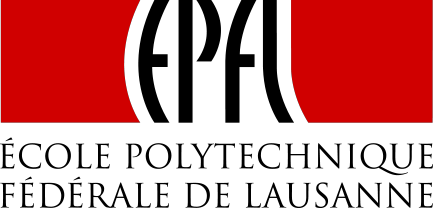
\includegraphics[width=5cm,height=2.4cm]{logo/EPFL.png}
\hspace{7cm}

\includegraphics[width=5cm,height=2.4cm]{logo/Shinshu.png}\\
\vspace{1cm}
\textsc{\large Laboratoire de Systèmes Robotiques, EPFL}\\[0.3cm] 
\textsc{\Large And}\\[0.3cm] 
\textsc{\large Faculty of Textile Science and Technology, Shinshu University}\\[0.5cm] % Major heading such as course name
\vspace{3cm}

{ \huge \bfseries Projet de Master 2017\\
\large Section de Microtechnique\\[1.5cm]
\HRule \\[0.4cm]
\LARGE Formation Control of Multiple Small Quadrotors by Using Model Predictive Control} % Title of your document
\HRule \\[1.5cm]
 
\Large Loïc \textsc{Dubois}\\ % Your name
\vspace{2.5cm}

\begin{minipage}[t]{0.4\textwidth}
\begin{flushleft} \large
\emph{Professors:} \\
Hannes \textsc{Bleuler}\\ % Supervisor's Name
Satoshi \textsc{Suzuki}\\ % Supervisor's Name
\end{flushleft}
\end{minipage}
~
\begin{minipage}[t]{0.4\textwidth}
\begin{flushright} \large
\emph{Assistant:} \\
Romain \textsc{Baud}\\ % Assistant's Name
\end{flushright} 
\end{minipage}\\[3cm]

{\large \today}\\ % Date, change the \today to a set date if you want to be precise


\vfill % Fill the rest of the page with whitespace

\end{titlepage}

\newpage
$\ $
\thispagestyle{empty}
%---------------------------------------------------------------------------------------
%	PRESENTATION SHEET
%----------------------------------------------------------------------------------------
\newpage
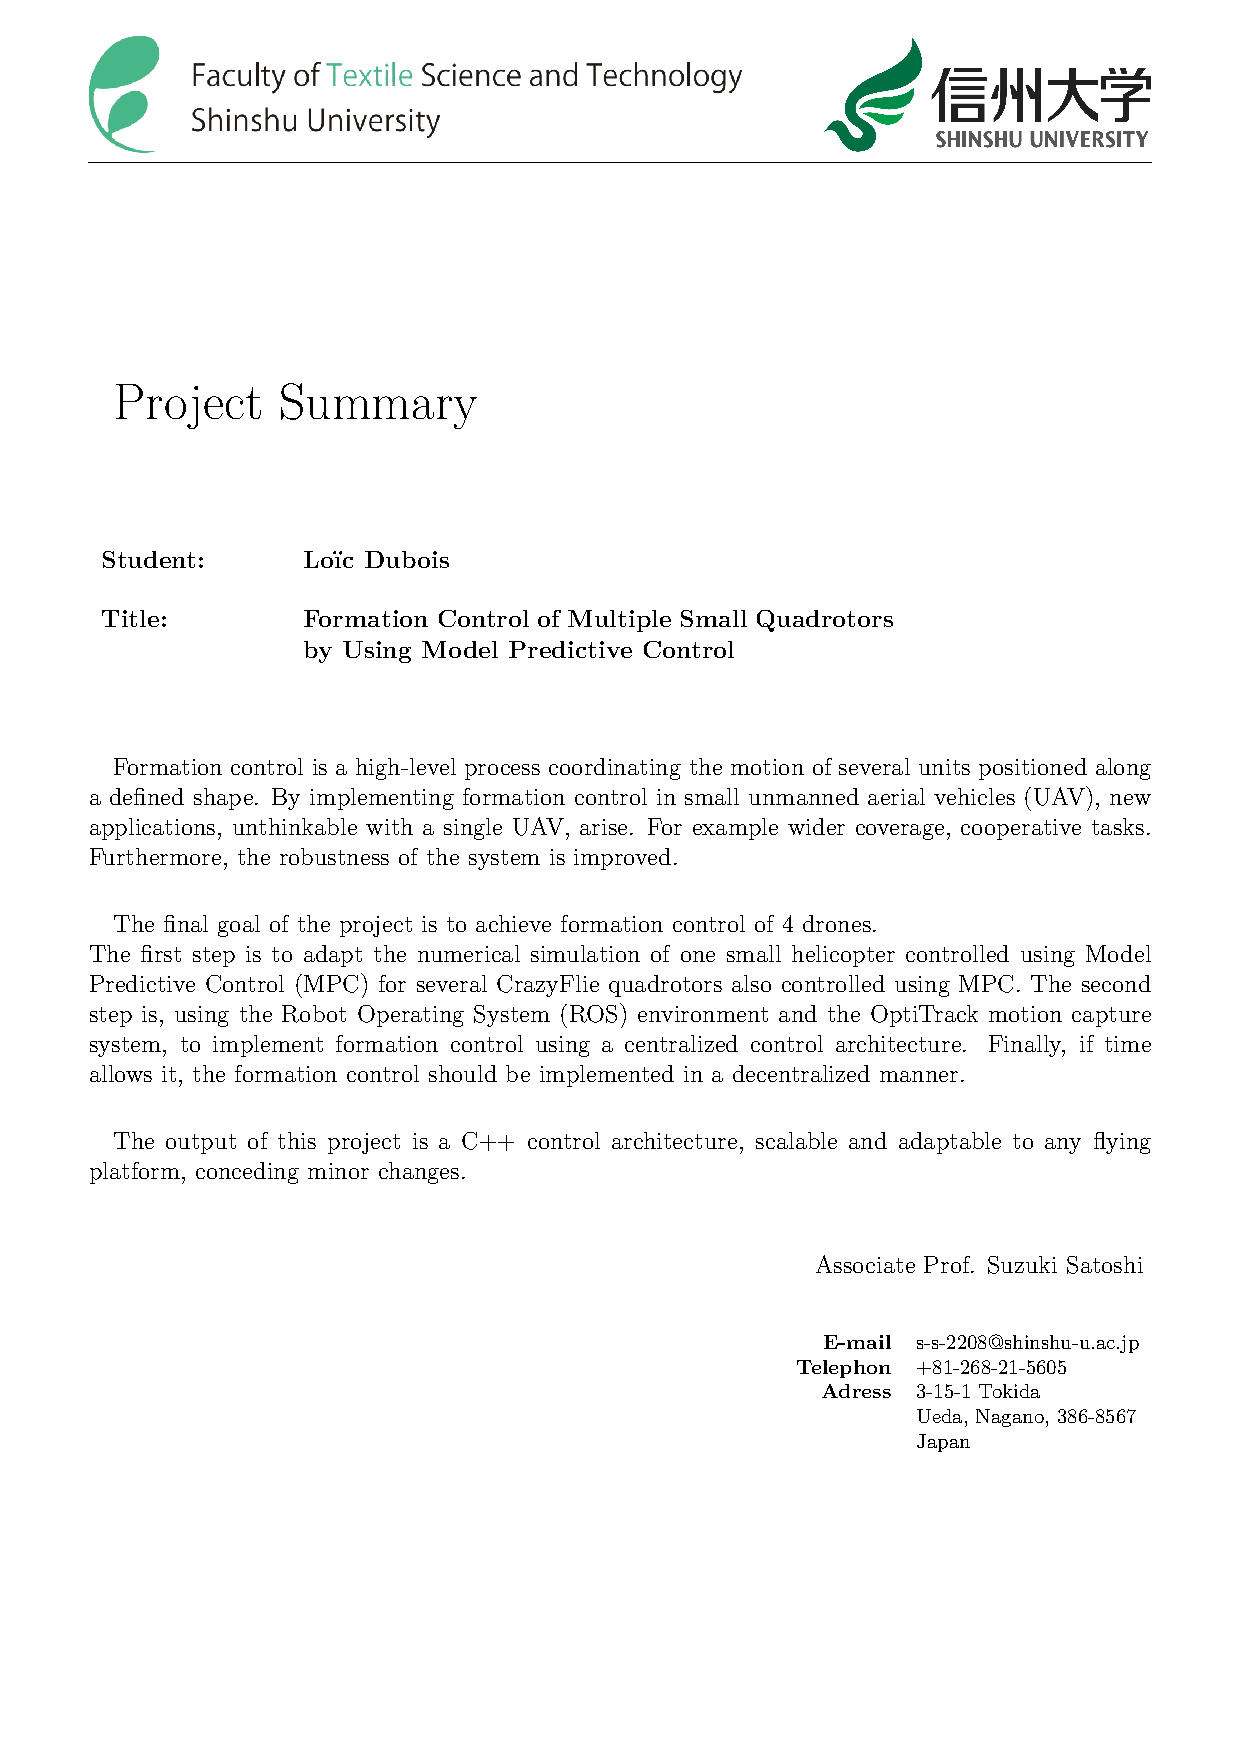
\includepdf{Presentation_sheet/Presentation_sheet.pdf}
\thispagestyle{empty}
\newpage
$\ $
\thispagestyle{empty}
%---------------------------------------------------------------------------------------
%	SUMMARY
%----------------------------------------------------------------------------------------
\newpage
%\includepdf{Presentation_project.pdf}
\textcolor{red}{SUMMARY - To be included - Template: c.f.: Project instructions, STI-MT website}
\thispagestyle{empty}
\newpage
$\ $
\thispagestyle{empty}
%---------------------------------------------------------------------------------------
%	TOC
%----------------------------------------------------------------------------------------
\newpage
\tableofcontents
\thispagestyle{empty}

%---------------------------------------------------------------------------------------
%	REPORT
%----------------------------------------------------------------------------------------
\newpage
% Numbering style
\pagenumbering{roman} 

\section*{Symbols and Abbreviations}
\addcontentsline{toc}{section}{Symbols and Abbreviations}
\subsection*{Symbols}
\begin{table}[h]
\centering
\begin{tabular}{p{8cm} p{8cm}}
$v$ \dotfill & A scalar \\
$\dot v$ \dotfill & First-order time derivative of scalar $v$ \\
$ \ddot v$ \dotfill & Second-order time derivative scalar $v$\\
$c_{\alpha}$ \dotfill & Cosine of angle $\alpha$ \\
$s_{\alpha}$ \dotfill & Sine of angle $\alpha$ \\
$\boldsymbol{v}$ \dotfill & A vector in world frame \\
$\boldsymbol{v}_B$ \dotfill & A vector in body frame \\
$\norm{\boldsymbol{v}}$ \dotfill & $L^2$ norm of vector $\boldsymbol{v}$ \\
$\boldsymbol{v}_{i:j}$ \dotfill & Sub-vector of components  \emph{i} to \emph{j} of vector $\boldsymbol{v}$\\
$V$ \dotfill & A matrix \\
$V^T,\boldsymbol{v}^T$ \dotfill & Transpose of a matrix $V$ or a vector $\boldsymbol{v}$ \\
$\phi$ \dotfill & Roll angle \\
$\theta$ \dotfill & Pitch angle \\
$\psi$ \dotfill & Yaw angle \\
$\boldsymbol{x}$ \dotfill & State vector \\
$\boldsymbol{u}$ \dotfill & Input vector \\
$\boldsymbol{x}_s$, $\boldsymbol{u}_s$ \dotfill & Working point subscript \\
$\boldsymbol{x}_r$, $\boldsymbol{u}_r$ \dotfill & Reference subscript \\
$A$ \dotfill & A matrix \\
$B$ \dotfill & B matrix \\
$C$ \dotfill & C matrix \\
$D$ \dotfill & D matrix \\
\end{tabular}
\end{table}

\subsection*{Abbreviations}
\begin{table}[h]
\centering
\begin{tabular}{p{8cm} p{8cm}}
MPC \dotfill & Model Predictive Control \\
NMPC \dotfill & Nonlinear Model Predictive Control \\
IP \dotfill & Interior Point \\
LP \dotfill & Linear Programming \\
QP \dotfill & Quadratic Programming \\
LQP \dotfill & Linearly Constrained QP \\
SQP \dotfill & Sequential Quadratic Programming \\
KKT \dotfill & Karush–Kuhn–Tucker conditions \\
GMRES \dotfill & Generalized Minimum Residual method \\
C/GMRES \dotfill & Continuation-GMRES method \\
ROS \dotfill & Robot Operating System \\
FPS \dotfill	 & Frame Per Second \\
PWM \dotfill & Pulse Width Modulation \\
IMU \dotfill & Inertial Measurement Unit \\
IR \dotfill & Infrared \\
\end{tabular} 
\end{table}

\newpage
\addcontentsline{toc}{section}{\listtablename}
\listoftables

\newpage
\addcontentsline{toc}{section}{\listfigurename}
\listoffigures

\newpage
% paragraph indentation and spacing
\setlength{\parskip}{1.5em}
\setlength{\parindent}{1em}
% Numbering style
\pagenumbering{arabic} 
\setcounter{page}{1}

\section{Introduction}
Build as a continuation of \cite{Suzuki2014}

\newpage
\section{Setup}
\begin{figure}[htbp]
\centering
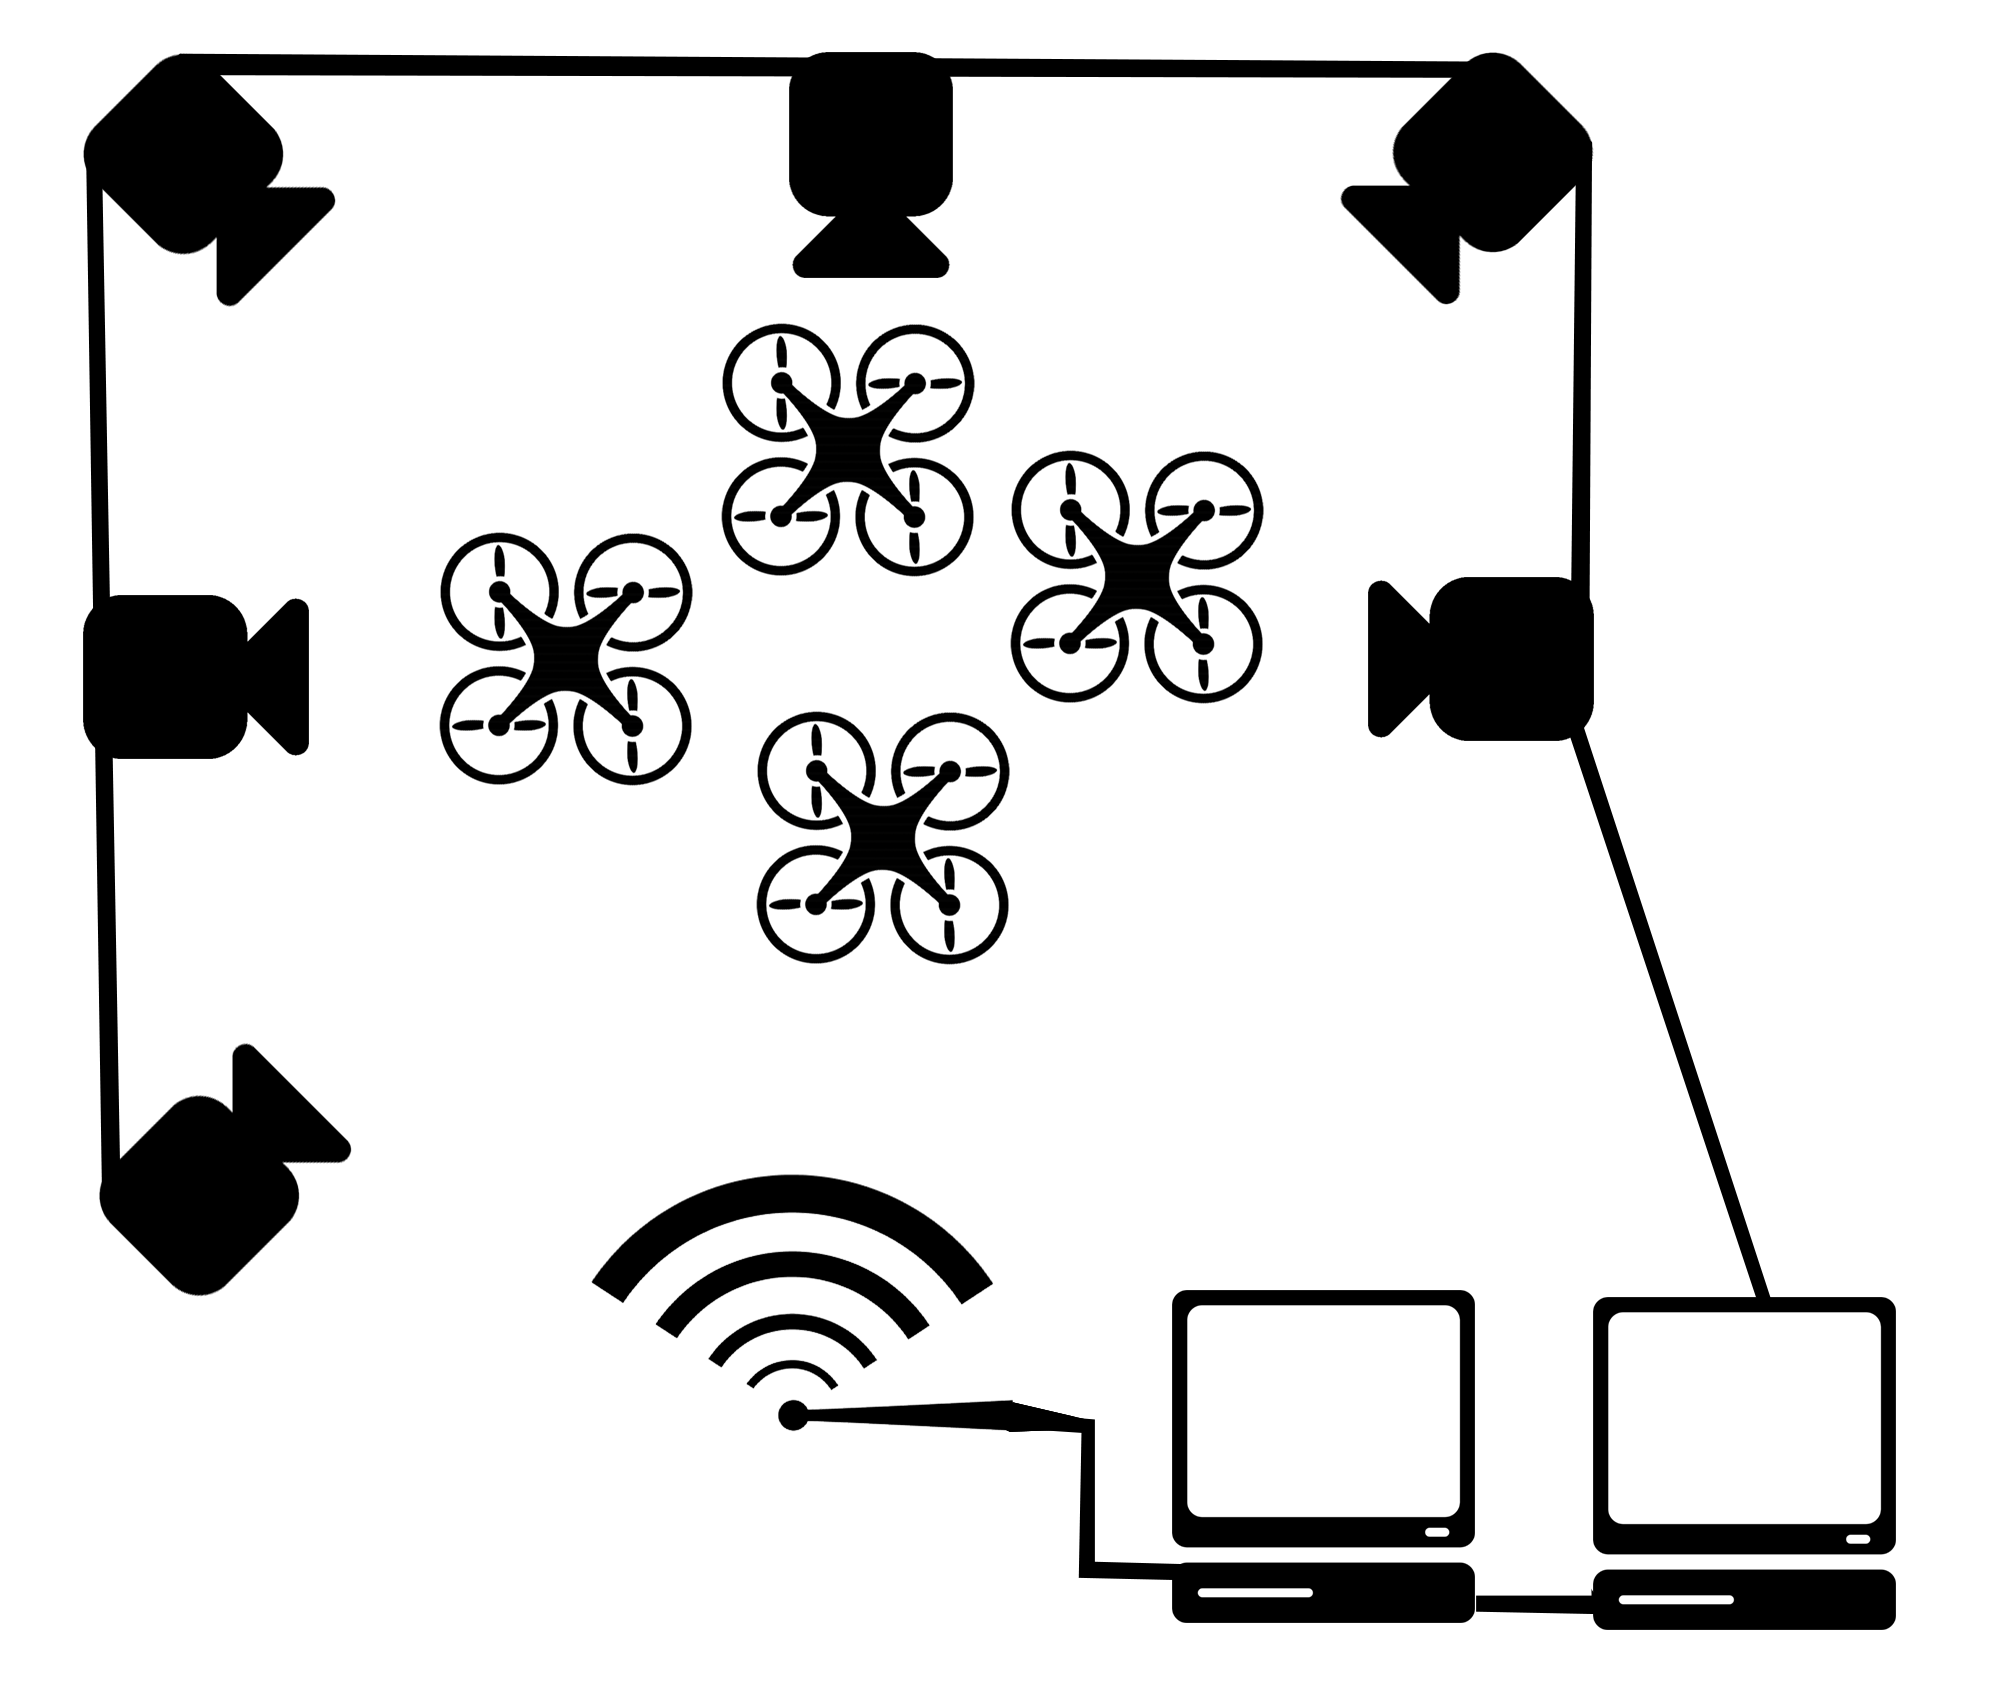
\includegraphics[width=.7\textwidth]{Images/setup}
\caption{Overview of the complete setup}
\label{fig:setup}
\end{figure}
The drones are flying in a motion capture environment, composed of several IR cameras and an independent PC This is system is able to provide information on the position and the attitude of the robot at a rate of \textcolor{red}{245} \emph{Hz}. On another PC, one, or several, controllers run at a frequency of 100 \emph{Hz}. The output of the controller is a vector of command sent to four quadrotors also at 100 \emph{Hz} through two radio dongles. On each quadrotor a second loop of controllers run at  500 \emph{Hz}. The quadrotors can also send information to the controller PC at rates up to 100 \emph{Hz}.

\subsection{Crazyflie 2.0 Quadrotor}
The Crazyflie 2.0 (or, to lighten notation, simply Crazyflie) is the second model of small quadrotor (or quadcopter or, simply, quad) developed by Swedish company, BitCraze \cite{bitcraze}. Its length of 92 millimeters from rotor to rotor and its weight of 27 grams make it a safe indoor flying machine. Moreover its on-board battery, allowing flights up to 7 minutes, can easily be replaced. Flights can be controlled either by an on-board long-range radio receiver and the appropriate emitter, the CrazyRadio PA, or thanks to a Bluetooth LE (low-energy) connexion and a smartphone with the dedicated application. The quadrotor is also equipped with multiple sensors, including a IMU with a 3-axis high-performance gyros and accelerometers , as well as a 3-axis magnetometer and a barometer.

The Crazyflie runs on an open source firmware, available on BitCraze website\cite{bitcraze}, making an ideal platform for academics researching and/or testing control, estimation, navigation or others algorithm. The code can easily be adapted, modified or improved without restrictions. A description of the core of the C control modules is given in section~\ref{sec:innerControl}. Note that the current firmware allows to log state and/or sensor data at a maximal rate of 100 \emph{Hz} and the Python client allows to export them to a CSV file, which can be read by Matlab, for example.

\begin{figure}[htbp]
\centering
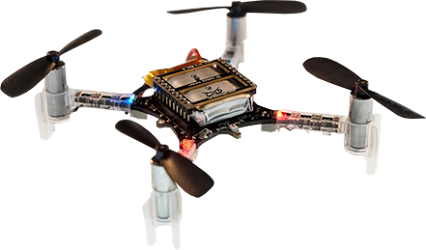
\includegraphics[width=.4\textwidth]{Images/crazyflie}
\captionsetup[subfloat]{labelformat=empty}
\subfloat[Picture from \cite{bitcraze}]{\hspace{\linewidth}}
\caption{The CrazyFlie quadrotor from BitCraze}
\label{fig:cf}
\end{figure}

\subsection{OptiTrack Motion Capture System}
The motion capture system consists, on one side, of eight Prime 13 cameras from OptiTrack and, on the other side, Motive:Tracker, a motion analysis software also from OptiTrack, capable of performing all steps from calibration to the motion capture itself, including also the exportation of the recorderd data.
This system allow a frame rate of 240 FPS and capture the drone position and attitude, or orientation using infrared markers. The camera latency is said to be 4.2 \textit{ms} (i.e.: approximately 1 frame in terms of FPS). The resolution of the motion capture system was measured in different points of the experiment room and are given below.

\subsection{Robot Operating System}
Robot Operating System, or ROS, is an open source suite of tools, libraries and software to develop robotic applications. From drivers to the most complex algorithm, it can handle any task, and on a very wide variety of platforms, including the Crazyflie \cite{Hoenig2015}. A vast worldwide community of developers has provided numerous modules, accessible free-of-charge, thus the development of educational, professional or research application is eased and fastened.

With ROS, each executable is called a node and communicate with other nodes through topics using a publisher/subscriber model. Communications is also implemented through a service/client model in which a request is send before receiving data. Code can either be written in C/C++ or Python and nodes does not need to run on the same platform to communicate with each others.

In the presented setup, the motion capture in his entirety is a node \textcolor{red}{with or without the state estimator?}, each of the four communication link is a node and depending on the implementation, there is one or four nodes for the controllers.


\newpage
\section{Quadrotor Dynamics}
A quadrotor can fly in two different configurations, they are commonly called $+$ (plus) and $\times$ (cross). In a $+$ configuration. The X- and the Y-axes are aligned with two perpendicular arms, the control is easier because only two propellers require to have their speed changed to move along one of the main axis. On the other side, a $\times$ configuration require all the propellers to change their speed. However the variation of speed per motor is smaller. In the following section, all dynamics equations are derived for a $+$ configuration. To fly in $\times$, minor changes have to be performed.

\subsection{State Representation}
To derive the equation of dynamics of a quadrotor, two reference frames are required, a world one (with index W or without index in the following equations) and the body one (always with index B).

 The body frame has its origin $O_B$ at the center of mass of the quadcopter, the X-axis is pointing towards the motor M1 and the Y-axis is pointing towards the motor M2, in case of $+$ configuration. In $\times$ configuration, the X-axis is pointing between the motors M1 and M4 and the Y-axis is pointing between the motors M1 and M2. Therefore, in both cases, the Z-axis is pointing downwards when the quadcopter lies on the floor (c.f.: figure~\ref{fig:frames}). 
The world frame origin is orientated such that its origin $O$ is in the center of the experiment room and its XY-plan corresponds to the floor. Furthermore, the X- and Y-axes are oriented in order to have the Z-axis is pointing downwards as well. 

\begin{figure}[htbp]
\centering
\subfloat[Body frame in $+$ configuration]{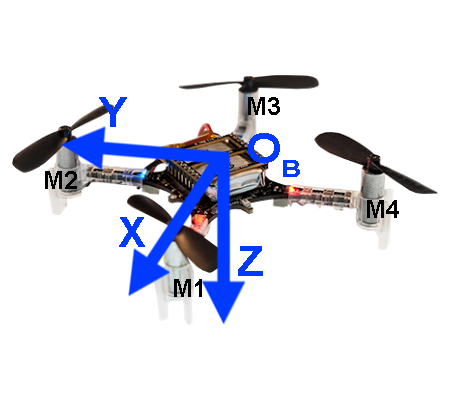
\includegraphics[width=.4\textwidth]{Images/frameBody}\label{fig:frameBody}}
\hspace{0.5cm}
\subfloat[Body frame in $\times$ configuration]{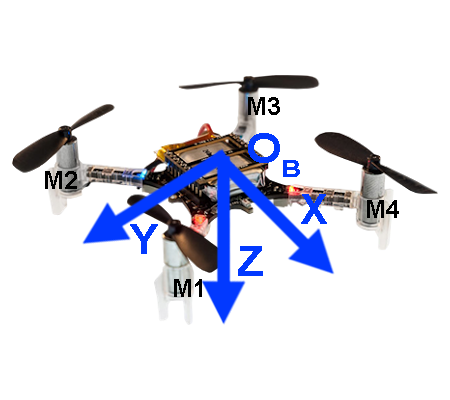
\includegraphics[width=.4\textwidth]{Images/frameBodyX}\label{fig:frameBodyX}}
\caption{Body frames in the two main configurations}
\label{fig:frames}
\end{figure}
  
Dynamics are derived using a 12-variables state description of the Crazyflie with the following state vector: the position of $O_B$ with respect to the world-frame, the speed of $O_B$ with respect to the world-frame and  the attitude angles (Euler angles) and the angular speed along the body axes:
 \[\boldsymbol{x} =  [x \ y \ z \ \dot x \ \dot y \ \dot z \ \phi \ \theta \ \psi \ \omega_{xB} \ \omega_{yB} \ \omega_{zB}]^T \]

When the Crazyflie is at the origin of the world frame, without flying and the axes of both frames are aligned, the state is:
 \[\boldsymbol{x} =  [0 \ 0 \ 0 \ 0 \ 0 \ 0 \ 0 \ 0 \ 0 \ 0 \ 0 \ 0 ]^T\]
 
This is a simple model considering translations and rotations along three axes. Some more advanced models can also include also the accelerometers biases, the gyroscopes drift, disturbances, making easily a 20-or-more-states description of a drone. But this is behind the scope of this project.

\subsubsection{Attitude Representation}
The attitude can be defined as the relative orientation of the body-frame with reference to the world frame and, nowadays, it can be expressed in various ways \cite{Diebel2006}. Among these representations, Euler angles, rotation matrices and unit quaternions are the most used. In order to derive the dynamics equations, the first two are required. Note, that the last one, unit quaternions, is implemented in the firmware for attitude estimation.

As stated in the previous subsection, the state of the drone is partially composed by its attitude expressed in Euler angles. These angles are the values of three ordered rotations around three main axes in space and the sequence of the three axes around which, each rotation is performed, defines the sub-representation.  Officially, there is 12 valid sub-representations but two are considered as the main ones: the $(3,1,3)$ sequence and the $(1,2,3)$ sequence. The first one, also known as the \emph{x-convention}, is often used in the study of spinning objects. The angles are called, in order, \emph{spin}, \emph{nutation} and \emph{precession}. The second one, commonly found in aerospace engineering, computer graphics and this project, is often also called \emph{Cardan angles}, \emph{Tait-Bryan angles} or \emph{nautical angles}. In this sub-representation, angles are called as follow \emph{bank}, \emph{attitude}, \emph{heading} or \emph{roll}, \emph{pitch}, \emph{yaw}. The latter is preferred. 

First the angle of rotation around the X-axis in the body frame defines the roll angle $\phi$ , then the rotation around the Y-axis defines the pitch angle $\theta$ and finally the rotation around the the Z-axis defines the yaw angle $\psi$. When applied in this order, rotations map a vector in the body-frame to the world-frame. The order of the axes $(X,Y,Z)$ is what gives this sub-representation its name $(1,2,3)$. On the figure~\ref{fig:attitude}, the roll angle corresponds to the rotation between the x''y''z'' and x'y'z' frames, the pitch x'''y'''z''' and x''y''z'' and the yaw xyz and x'''y'''z'''.
\[\boldsymbol{q} =  \begin{bmatrix} \phi \\ \theta \\ \psi \end{bmatrix}\]

Although, Euler angles are easy to visualize, they are not suitable for fast computation of 3D-rotations. Likewise, they suffer from singularities. For example, In the case of a pitch angle $\theta=90\degree$, variation in yaw angle are indistinguishable from variation in roll angle. Nonetheless, these are extreme cases that are never met in the scope of this project.

\begin{figure}[htbp]
\centering
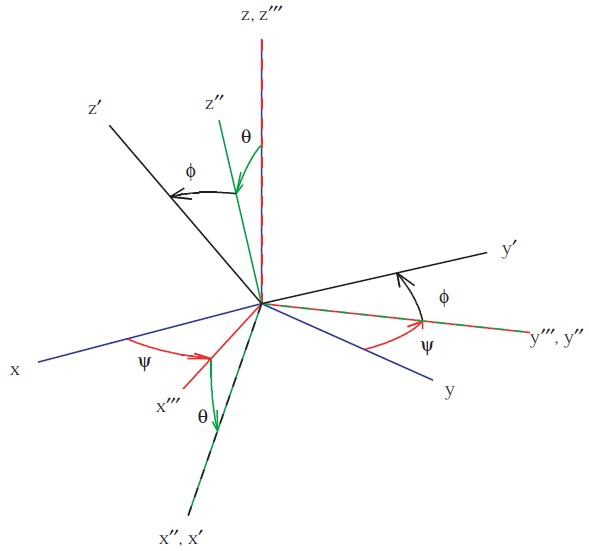
\includegraphics[width=0.5\textwidth]{Images/attitude}
\captionsetup[subfloat]{labelformat=empty}
\subfloat[Drawing from \cite{Diebel2006}]{\hspace{\linewidth}}
\caption{Roll $\phi$, Pitch $\theta$ and Yaw $\psi$ Angles}
\label{fig:attitude}
\end{figure}

Another possibility to represent attitude is with a rotation matrix. This matrix maps is very useful to compute the mapping between the body frame and to the world frame. The reverse operation can be easily computed, as the all the matrix rotations are part of the special orthogonal group $SO(3)$, their inverse is also their transpose.
\[ \boldsymbol{v_B} = R_{BW} \boldsymbol{v_W}\]
\[ \boldsymbol{v_W} = R_{WB} \boldsymbol{v_B}\]
\[ R_{BW} = R_{WB}^{-1} = R_{BW}^T \]

Each rotation in the 3-dimensional space can be decomposed in three rotations around the three main axes:
\[R_{Ox}(\alpha)  = \begin{bmatrix} 1 & 0 & 0 \\ 0 & \cos{\alpha} & \sin{\alpha} \\ 0 & -\sin{\alpha} & \cos{\alpha}  \end{bmatrix} R_{Oy}(\beta)  = \begin{bmatrix} \cos{\beta} & 0 & -\sin{\beta} \\ 0 & 1 & 0 \\ \sin{\beta} & 0 & \cos{\beta}  \end{bmatrix} R_{Oz}(\gamma)  = \begin{bmatrix} \cos{\gamma} & \sin{\gamma} & 0 \\ -\sin{\gamma} & \cos{\gamma} & 0 \\ 0 & 0 & 1  \end{bmatrix} \]

Moreover, consecutive rotations can be easily combined by left-multiplying the matrices. Despite its simplicity, this representation requires nine variable. Therefore, Euler angles are preferred for representation and an easy conversion to rotation matrix is performed for computation purposes. The mapping between Euler angles and rotation matrix, consisting of the multiplication of the three individual rotation matrices in the right order, and is computed as follow ($c_\alpha$ corresponds to $\cos{\alpha}$ and $s_\alpha$ to $\sin{\alpha}$):
\[R_{BW}(\phi, \theta, \psi)= R_{Ox}(\phi) R_{Oy}(\theta) R_{Oz}(\psi)  = 
\begin{bmatrix}  c_\theta c_\psi  & c_\theta s_\psi  & -s_\theta  \\ s_\phi s_\theta c_\psi -c_\phi s_\psi  & s_\phi s_\theta s_\psi  + c_\phi c_\psi  & c_\theta s_\phi  \\ c_\phi s_\theta c_\psi +s_\phi s_\psi  & c_\phi s_\theta s_\psi -s_\phi c_\psi  & c_\theta c_\phi  \end{bmatrix} \]

Finally the last convention is the unit quaternion. The unit quaternion is a 4-dimensional generalization of complex numbers whose norm $\norm{\boldsymbol{q}} = 1$.
\[ \boldsymbol{q} =  q_0 + q_1 \cdot i + q_2 \cdot j + q_3 \cdot k = \begin{bmatrix} q_0 \\ q_1 \\ q_2 \\ q_3 \end{bmatrix} = \begin{bmatrix} q_0 \\ q_{1:3} \end{bmatrix} \]

Although they benefit from most of the tools of complex algebra such as:
\[ \boldsymbol{\bar q} = \begin{bmatrix} q_0 \\ -\boldsymbol{q}_{1:3} \end{bmatrix},  \quad \norm{\boldsymbol{q}} = \sqrt{q_0^2 + q_2^2 + q_3^2 + q_4^2}, \quad \boldsymbol{q}^{-1} = \frac{\boldsymbol{\bar q}}{ \norm{\boldsymbol{q}}} \]
The multiplication is now non-commutative:
\[\boldsymbol{q} \cdot \boldsymbol{\lambda} = \begin{bmatrix} q_0p_0 - \boldsymbol{q}^T_{1:3}\boldsymbol{\lambda}_{1:3} \\ q_0\boldsymbol{\lambda}_{1:3} + p_0\boldsymbol{q}_{1:3} - \boldsymbol{q}_{1:3} \times \boldsymbol{\lambda}_{1:3} \end{bmatrix} \]
Equivalently, as with rotation matrices, a vector in the world frame can be mapped in the body frame:
\[ \begin{bmatrix} 0 \\ \boldsymbol{v_B} \end{bmatrix}  = \boldsymbol{q} \cdot \begin{bmatrix} 0 \\ \boldsymbol{v_W} \end{bmatrix} \cdot \boldsymbol{q}^{-1} \]

The attitude estimation algorithm on the Crazyflie uses quaternions, that are then mapped to Euler angles for control. A detailed explanation of the algorithm can be found in appendix ~\ref{app:att_estim}.

The weakness of unit quaternions is, especially in optimization problem like MPC, enforcing the quadratic constraints on the norm. Although several methods exist to ease this problem, unit quaternions still requires an additional variable than Euler angles and lack of meaning for the human mind.
\subsection{Newton-Euler Rquations}
\label{sec:dynamicsEquations}

\begin{figure}[htbp]
\centering
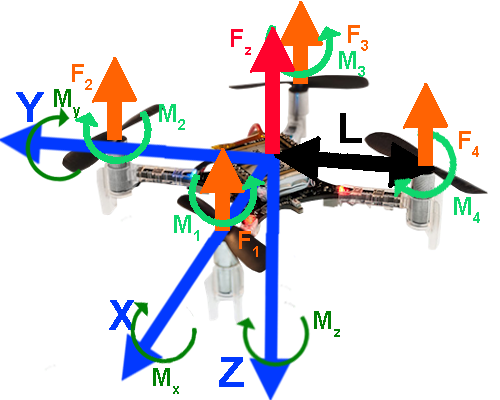
\includegraphics[width=0.5\textwidth]{Images/forceMoments}
\caption{Force and torques applied on the CrazyFlie}
\label{fig:forceMoment}
\end{figure}

In a quadcopter, each propeller generates a force $F_i$ and a torque $M_i$ proportional to the square of its spinning speed  (c.f.: figure~\ref{fig:forceMoment}). The vector $\boldsymbol{w}$ is the vector of the squared spinning rates, (sometime confusingly called thrust.
\[ \boldsymbol{w} = [\omega^2_1 \  \omega^2_2 \  \omega^2_3 \  \omega^2_4]^T \]
\[F_i =  K_f  w_i \ \ \ M_i = K_t  w_i  ,\  i = 1,2,3,4\]

In a ''\emph{plus}'' configuration, the thrust force (or simply thrust) $F_{z}$ and the torques $M_{x}, M_{y}, M_{z}$  applied to the center of mass of the quadrotor, depends on $\boldsymbol{w}$ and is computed as follow:
\[  
\begin{bmatrix}
F_{z}\\ 
M_{x}\\
M_{y}\\
M_{z}
 \end{bmatrix}_B
=
\begin{bmatrix}
-K_f & -K_f & -K_f & -K_f\\
0 & -K_f \cdot L & 0 & K_f \cdot L\\
K_f \cdot L & 0 & -K_f \cdot L & 0\\
-K_t & K_t & -K_t & K_t
\end{bmatrix}
\textbf{w} = K\textbf{w}
\]
Where $L$ is the distance from the axis of rotation of a motor and $O_b$.

The dynamics equations can now be derived using Newton-Euler equations:
\[ m\boldsymbol{\ddot r} =  \sum_i \boldsymbol{F_i} = \boldsymbol{G} + \boldsymbol{T} + \boldsymbol{D} = \begin{bmatrix}  0\\ 0\\ mg \end{bmatrix} + R_{BW}^T(\phi, \theta, \psi) \begin{bmatrix}  0\\ 0\\ -F_z \end{bmatrix}_B + \begin{bmatrix}  D_x\\ Dy\\ D_z \end{bmatrix}\]
\[ I\boldsymbol{\dot \omega_B} =  \sum \boldsymbol{M_B} - \boldsymbol{\omega_B}  \times (I \boldsymbol{\omega_B} )=  
\begin{bmatrix}  M_{x}\\ M_{y}\\ M_{z} \end{bmatrix}_B - \boldsymbol{\omega_B}  \times (I \boldsymbol{\omega_B}) \]
Where $\boldsymbol{r}$ is the position of $O_B$, expressed in the world frame,  $\boldsymbol{G}$ is the gravity force, $\boldsymbol{T}$ is the thrust force generated by the propellers, $\boldsymbol{D}$ is the drag force, $I$  is the inertia matrix of the quadcopter and $\boldsymbol{\omega_B}$ is the angular speed in the body frame.

In order to link the attitude angle rates to body rate, the matrix $W(\phi,\theta,\psi)$ is still required: %Note for me: In reference document, the matrix is [E']^{-1}
\[ W(\phi,\theta,\psi) = \begin{bmatrix}  1 & \sin\phi \tan\theta  & \cos\phi \tan\theta \\ 0 & \cos\phi  &-\sin\phi  \\ 0 & \frac{\sin\phi }{\cos\theta } & \frac{\cos\phi }{\cos\theta } \end{bmatrix}\]
\[ \boldsymbol{ \dot q} = \begin{bmatrix} \dot \phi \\ \dot \theta\\ \dot \psi \end{bmatrix} = W(\phi,\theta,\psi) \boldsymbol{\omega_B}\]

\subsection{Model}
 \[ \boldsymbol{x} =  [x \ y \ z \ \dot x \ \dot y \ \dot z \ \phi \ \theta \ \psi \ \omega_{xB} \ \omega_{yB} \ \omega_{zB}]^T \]
 \[ \boldsymbol{w} = [\omega^2_1 \  \omega^2_2 \  \omega^2_3 \  \omega^2_4]^T \]
\[\left\{ \begin{matrix}[l]
\begin{bmatrix} \dot x_{1}\\\dot x_{2} \\ \dot x_{3} \end{bmatrix} = \begin{bmatrix}  x_{4}\\ x_{5} \\ x_{6} \end{bmatrix}\\
\begin{bmatrix} \dot x_{4}\\\dot x_{5} \\ \dot x_{5} \end{bmatrix} = \frac{1}{m}(\begin{bmatrix}  0\\ 0\\ mg \end{bmatrix} + R_{BW}^T(x_7, x_8, x_9) \begin{bmatrix}  0\\ 0\\ F_{z}(\boldsymbol{w}) \end{bmatrix}_B + \begin{bmatrix}  D_x\\ D_y\\ D_z \end{bmatrix})\\
\begin{bmatrix} \dot x_{7}\\\dot x_{8} \\ \dot x_{9} \end{bmatrix} = W(x_7, x_8, x_9)\begin{bmatrix}  x_{10}\\ x_{11} \\ x_{12} \end{bmatrix} \\
\begin{bmatrix} \dot x_{10}\\\dot x_{11} \\ \dot x_{12} \end{bmatrix} = I^{-1}(\begin{bmatrix}  M_{x}(\boldsymbol{w})\\ M_{y}(\boldsymbol{w})\\ M_{z}(\boldsymbol{w}) \end{bmatrix}_B - \begin{bmatrix}  x_{10}\\ x_{11} \\ x_{12} \end{bmatrix} \times (I\begin{bmatrix}  x_{10}\\ x_{11} \\ x_{12} \end{bmatrix}))\\
\end{matrix} \right.\]

\newpage
\section{High-Level Control - Formation Control}
Collective movement is a widely observed phenomenon in both natural and civilized worlds. In animal societies, the phenomenon, called flocking, herding, schooling or swarming, depending on the species, happens for all size of groups, from tiny insects to huge mammals, in homo- or heterogeneous groups and sometimes can be circumstance-driven, like migrations. A flock, generally used to describe any of the denomination introduced before, is characterized by directed movement and quick reactions to obstacle at the global scale, even though there is apparent leading mechanism. Among the benefits of group motion, dilution of risk, improved exploration, foraging and sensing capabilities, energy saving are the most interesting. Of course costs arise also from group formation like the diminution of resource per capita but these concern mostly living entities \cite{Krause2002, Parrish1997}. Flocks principle have been successfully implemented in robotics and are a excellent example of swarm intelligence, in which global structure appears solely through numerous local interactions \cite{Bonabeau1999, Reynolds1987}. Indeed, computing trajectories for every robots, taking into account other robots, obstacles and some other constraints can easily on become intractable, even for the best computers, when the number of robots increase. 

However, another kind of collective movement exists, motion in formation. Compared to flocking, where the relative location and the neighborhood of an individual is in permanent evolution, motion in formation assigns a specific position to each member and its neighborhood becomes static (except upon failure of a member of the group or reconfiguration). In natural societies, V-shape flights of birds is a good example. Despite the precise positioning of every members, formation control can also be implemented following swarm intelligence principles. While flocking benefits more from robustness, flexibility and scalability, formations are more efficient, require less individuals for an equivalent coverage and are more intuitively commanded. Of course, the ideal group configuration depends on the application, the environment and the type and the number of robot. In this work, solely due to the number of available robots, the study of motion in formation will exclusively be studied.

In a more global perspective, a swarm of robots, compared to a single robot achieving a similar task, usually require simpler units, increase reliability \cite{Beni2004} and allows for reconfigurability and more flexibility. Therefore swarm members result in simpler hardware, software, as well as sensing, acting and communicating capabilities. But, on the other side, the cost of robustness is efficiency, in terms of time, total energy required or eventually another metrics. In summary, swarm robotics is a careful balance between exploration et exploitation behaviors, whose application will emphasize one or the other.

\subsection{Formation Taxonomy}
When studying formations, they can be classified in two categories: \emph{virtual structure} and {leader-follower} \cite{Chen2005, Arkin1999}. Each of them can subsequently be divided in several sub-categories.
\begin{itemize}
\item \emph{Leader-follower:} In leader-follower, each follower robot is assigned one or several leaders and use them as reference to define its position in the formation. The main sub-category is \emph{leader-referenced} formations (c.f.: figure~\ref{fig:leader}). In this case, the reference is a unique member for the whole the group, called the leader. When there is several leaders, the formation is also often referred to as \emph{neighbor-referenced formation}  (c.f.: figure~\ref{fig:neighbor}). Additionally, it is also possible to define a formation leader, which has no leader in the formation \cite{Mataric2002} (c.f.: figure~\ref{fig:neighborLeader}).
\item \emph{Virtual structure:} In a virtual structure formation, the reference point(s) is(are) not linked to any physical member of the group. \emph{Unit-centered formation} \cite{Arkin1999} (c.f.: figure~\ref{fig:unitCenter}), is a special sub-category in which the reference corresponds to the center of mass of the formation. In \emph{purely virtual structure} (c.f.: figure~\ref{fig:virtual}) formations are based on \emph{a-priori} knowledge of the trajectory to follow and are characterized by no inter-robot interactions. 
\end{itemize}

Every configuration has its strengths and weaknesses. In \cite{Arkin1999}, it is stated that unit-centered and leader-referenced formations perform better than neighbor-referenced ones. Furthermore, a lot of experimentation relies on leader-referenced \cite{Manikonda1999,Lim2009,Fukushima2013,Shin2009, Zhao2014} or virtual structure \cite{Dunbar2002,Chao2011,Kuriki2015,Chao2012} (not necessarily unit-centered) formations. Nevertheless, neighbor-referenced is still sometimes considered \cite{Wang2007}.

From a more objective point of view, leader-referenced formations can easily include a human-controlled member in the group to drive the formation. But, on the other hand, the failure of the leader is  almost always fatal in case of leader-referenced and, in neighbor-referenced, the member at the end of consecutive leader-follower pairs is subject to the cumulative uncertainty of its predecessors. However, it is the configuration possibly requiring the smallest sensing/communication range if the leaders are chosen efficiently.
On the other side, virtual structure formations tends to act more tightly as a whole than a sum of individuals, which make it less performing for obstacle-avoidance applications but also achieving stronger formation. It is easy to drive purely virtual structure formations with a pre-computed trajectory that is simply shifted in space for every member but driving a formation without feedback can lead to huge errors and, depending on the measure metrics, not achieving formation at all \cite{Pugh2009}. In unit-centered, the feedback comes from the center of mass of the formation computation at every time step but driving the formation to a desired reference can also be tricky. Moreover, communications or sensing capabilities required can be high as every member requires knowledge of the state of every other member in the formation, which make this formation the worst in terms of amount of data required per member. Nevertheless, it can be seen as a positive trait if reconfiguration is required.

Considering carefully all these points, it has been decided to focus on \emph{leader-referenced} formations for both centralized and decentralized control and also \emph{neighbor-referenced} formations for decentralized control.

Note that the the shape of the formation could also be discussed in depths. Nonetheless, it felt like a highly application-dependent feature. Therefore the choice of a diamond shape is made without any particular reason. Below, list of few typical applications for each shape defined in \cite{Arkin1999} is provided:
\begin{itemize}
\item \emph{Line} : Coverage is maximized. Then ideal for search and rescue, cleaning or lawn-mowing, surveillance and patrolling and exploration.
\item \emph{Column} : Minimal width, high redundance. Military formation
\item \emph{Diamond} or \emph{square} : Tradeoff coverage-redundance. Well-suited for aerial-mapping, distributed sensing or monitoring
\item \emph{Wedge} : Military formation.
\end{itemize}

\begin{figure}[htbp]
\centering
\subfloat[A leader-referenced formation]{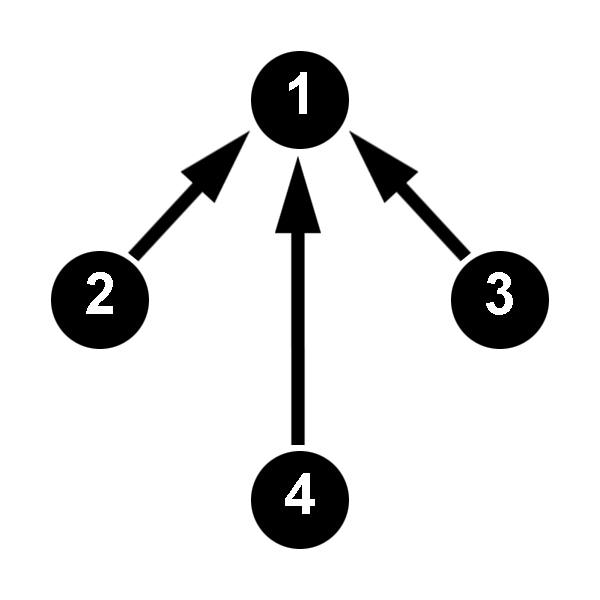
\includegraphics[width=.4\textwidth]{Images/graphLeader}\label{fig:leader}}
\hspace{10cm}
\subfloat[A neighbor-referenced formation]{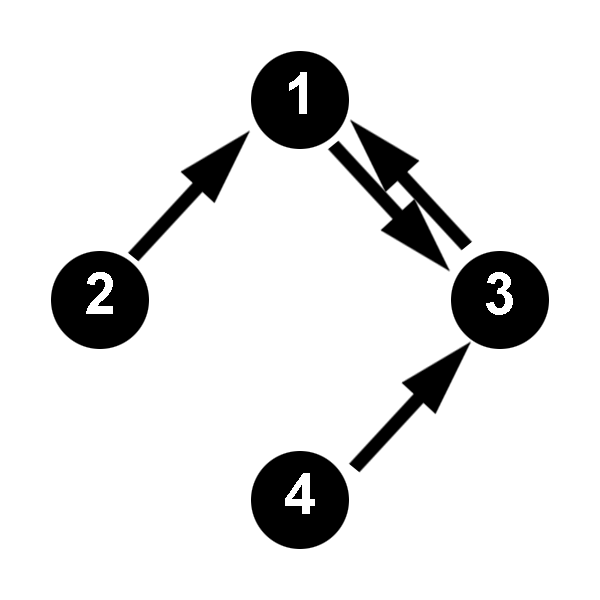
\includegraphics[width=.4\textwidth]{Images/graphNeighbor}\label{fig:neighbor}}
\hspace{0.2cm}
\subfloat[A neighbor-referenced formation with formation leader]{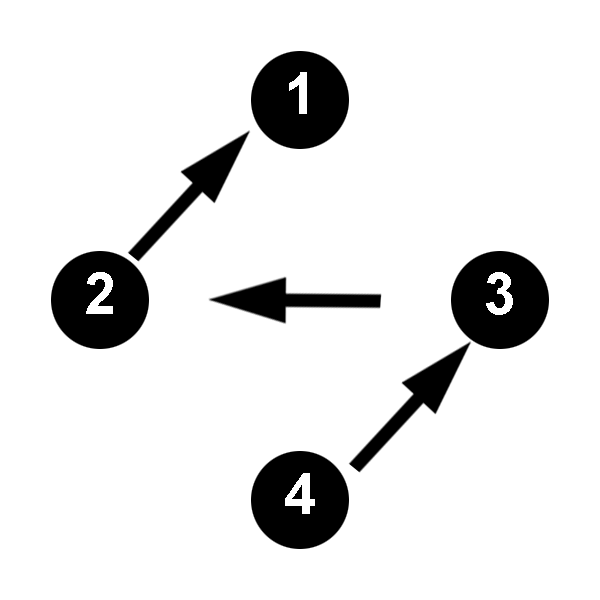
\includegraphics[width=.4\textwidth]{Images/graphNeighbor2}\label{fig:neighborLeader}}
\hspace{0.2cm}
\subfloat[A unit-centered formation]{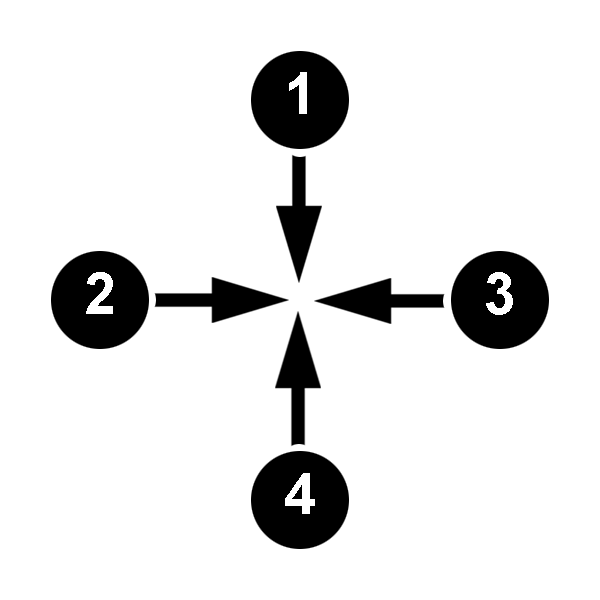
\includegraphics[width=.4\textwidth]{Images/graphUnitCenter}\label{fig:unitCenter}}
\hspace{0.2cm}
\subfloat[A purely virtual formation]{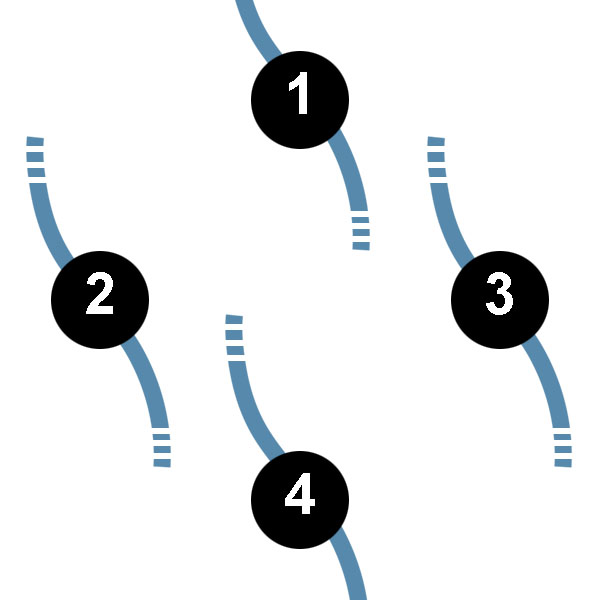
\includegraphics[width=.4\textwidth]{Images/graphVirtual}\label{fig:virtual}}
\hspace{0.2cm}
\caption{The taxonomy illustrated for a diamond-shaped formation}
\label{fig:graphs}
\end{figure}

\subsection{Control Architecture}
\subsubsection{Centralized, Decentralized and Distributed Control}

When several robots are evolving in the same environment or when they are performing collective tasks, such as flight in formation, controllers can be implemented in three different manners \cite{Scattolini2009}:
\begin{itemize}
\item \emph{Centralized}: In centralized control architectures, all the information is concentrated in one node, in our case, the formation controller. Depending on the system to control, such an implementation can be huge and computationally costly and requires good communication networks. Moreover, in a way similarly to leader-referenced formations, the failure of the central controller is fatal to the whole group. Nevertheless, the controller can make decision with complete informations about the system.
\item \emph{Distributed}: In this case, a central node is still present but the problem to solve is divided into smaller subproblems given to several controllers. This approach is often beneficial in terms of computation cost but still suffers from having a central node and if the sub-problems are coupled, approximations have to be made. The central node is often called coordinator or regulator.
\item \emph{Decentralized}: A decentralized architecture is characterized by the absence of a central node. While it is typically more robust, fault tolerant and scalable, the information on the whole system is limited and often more uncertain.
\end{itemize}

Given our setup, a purely decentralized implementation is impossible for several reasons. First, the Crazyflie is lacking sensing capabilities in order to relatively localize itself or other members of the group. Therefore a motion capture system is required, which is a sort of centralization. Then, all the controllers run off-board, on the same PC. \textcolor{red}{Processor powerful enough?}. 
However, decentralized control is simulated by several mechanisms
\begin{itemize}
\item \emph{Uncertain relative positioning}: Every position is expressed in the local frame whether for reference position or other drones positions. Furthermore, as sensors are theoretically always a bit different, a same distance can be seen differently for two distinct drones.
\item \emph{Local perception}: The sensing capability is limited in range, which mean that the position of other robots can be unavailable
\item \emph{Individual independent controllers}: There is as many controller as there are robots. Each one of them is running the same algorithm but communications between them is impossible.
\end{itemize}

Independently of the implementation, the control can be divided in two loops, the inner one and the outer one. The inner loop, or inner controller, implemented in the Crazyflie firmware, controls the roll and pitch angles, as well as the yaw rate. The outer loop is responsible for formation control and the collision avoidance. In figure~\ref{fig:controlArchi}, the architecture for both centralized and decentralized control is presented. Note that for decentralized, only one of the four controllers is shown.

\begin{figure}[htbp]
\centering
\subfloat[Centralized Control Architecture]{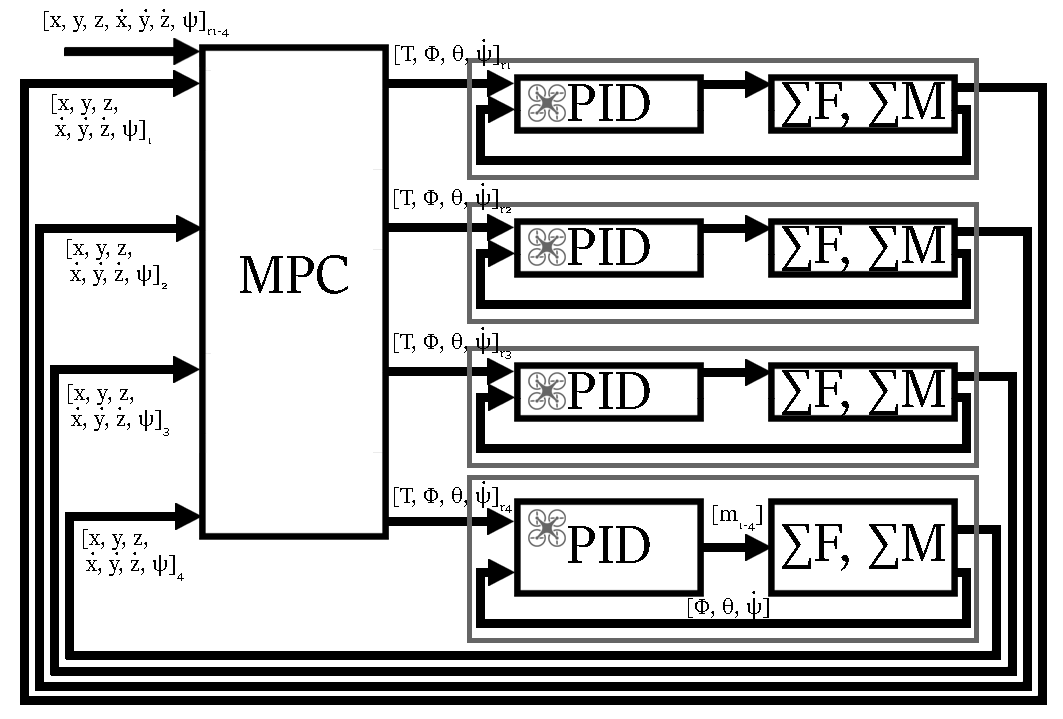
\includegraphics[width=1\textwidth]{Images/controlArchiCent}\label{fig:controlArchiCent}}
\hspace{0.2cm}
\subfloat[Decentralized Control Architecture]{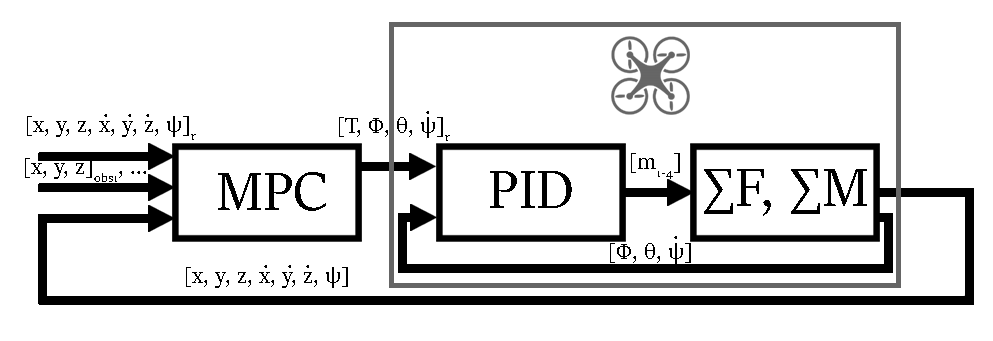
\includegraphics[width=1\textwidth]{Images/controlArchiDistrib}\label{fig:controlArchiDistrib}}
\caption{Graph-based controllers. The gray rectangle represent the part of the architecture running on the Crazyflie.}
\label{fig:controlArchi}
\end{figure}

\subsection{Fomation Controllers}

Formation control has been implemented in various ways among which, behavior-based control \cite{Arkin1999, Mataric2002, Pugh2009}, graph-based control  \cite{Gowal2013, Falconi2010} are the most common. Both of these methods can easily be implemented either in a centralized or in a decentralized manner for any of the configuration presented previously using relative localization sensors and IDs or communication. Another possibility, and the one explored in this project, consists of using an Model Predictive controller. It has already been successfully implemented for various type of formations, with and without collision avoidance \cite{Manikonda1999, Chao2011, Wang2007, Lim2009, Kuriki2015,Dunbar2002,Fukushima2013,Shin2009,Zhao2014,Chao2012}. At the price of heavier computational complexity, additional capabilities can be introduced in the controller formulation, such as obstacle and collision avoidance. In addition to that, it is the only method, among the three presented able to constrain the states or the input commands sent to the robot and to provide a prediction of the state trajectory.

Behavioral controllers, usually implemented using potential or force field (cooperative behaviors) \cite{Arkin1999, Pugh2009} or subsumption architecture (competitive behaviors) are an elegant way for designing reactive controllers for extremely simple units. Typically a behavior provides a force from which adequate input command can be derived. As stated before, although this approach can be implemented for any type of formation it is especially well adapted for leader-follower formations in which fewer communications or sensing is required. However, despite its ease of use, several drawbacks exist: existence of local minima (c.f.: figure~\ref{fig:potentialTraj}) and oscillatory motion mainly. Moreover, mathematical analysis is often difficult and the wanted result is not guaranteed. Indeed, adding an obstacle avoidance behavior often leads to poorer performances of the formation behavior \cite{Ren2004}. An example of potential could be the following (c.f.: figure~\ref{fig:potentialEx}).
\[ \dot r_i =  \left\{ \begin{matrix*}[l] 0 & if\ r_{f,i}-r_i\ \in [0; d_1] \\ \alpha(r_{f,i}-r_i-d_1) & if\ r_{f,i}-r_i\ \in [d_1; d_2] \\  \beta(r_{f,i}-r_i-d_2)^2 + \alpha(r_{f,i}-r_i-d_1) & if\ r_{f,i}-r_i\ \in [d_2; \inf] \end{matrix*} \right. \ for\ i = 1,2,3\]
Where $F_{f,i}$ is the reference position in formation, $r_i$ the current position in one dimension, $d_1$, $d_2$, $\alpha$ and $\beta$ are parameters

\begin{figure}[htbp]
\centering
\subfloat[A trajectory in a potential field with local minima]{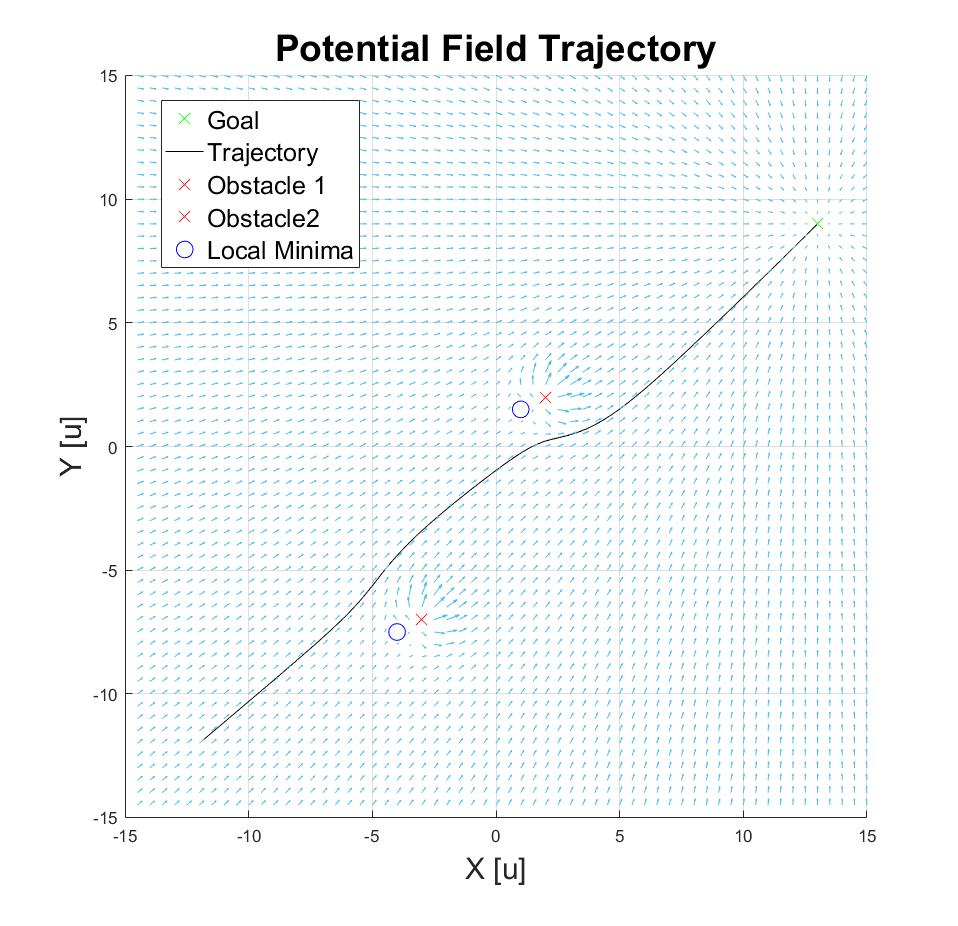
\includegraphics[width=.5\textwidth]{Images/potentialTraj}\label{fig:potentialTraj}}
\subfloat[An example of 1-D potential field with dead zone]{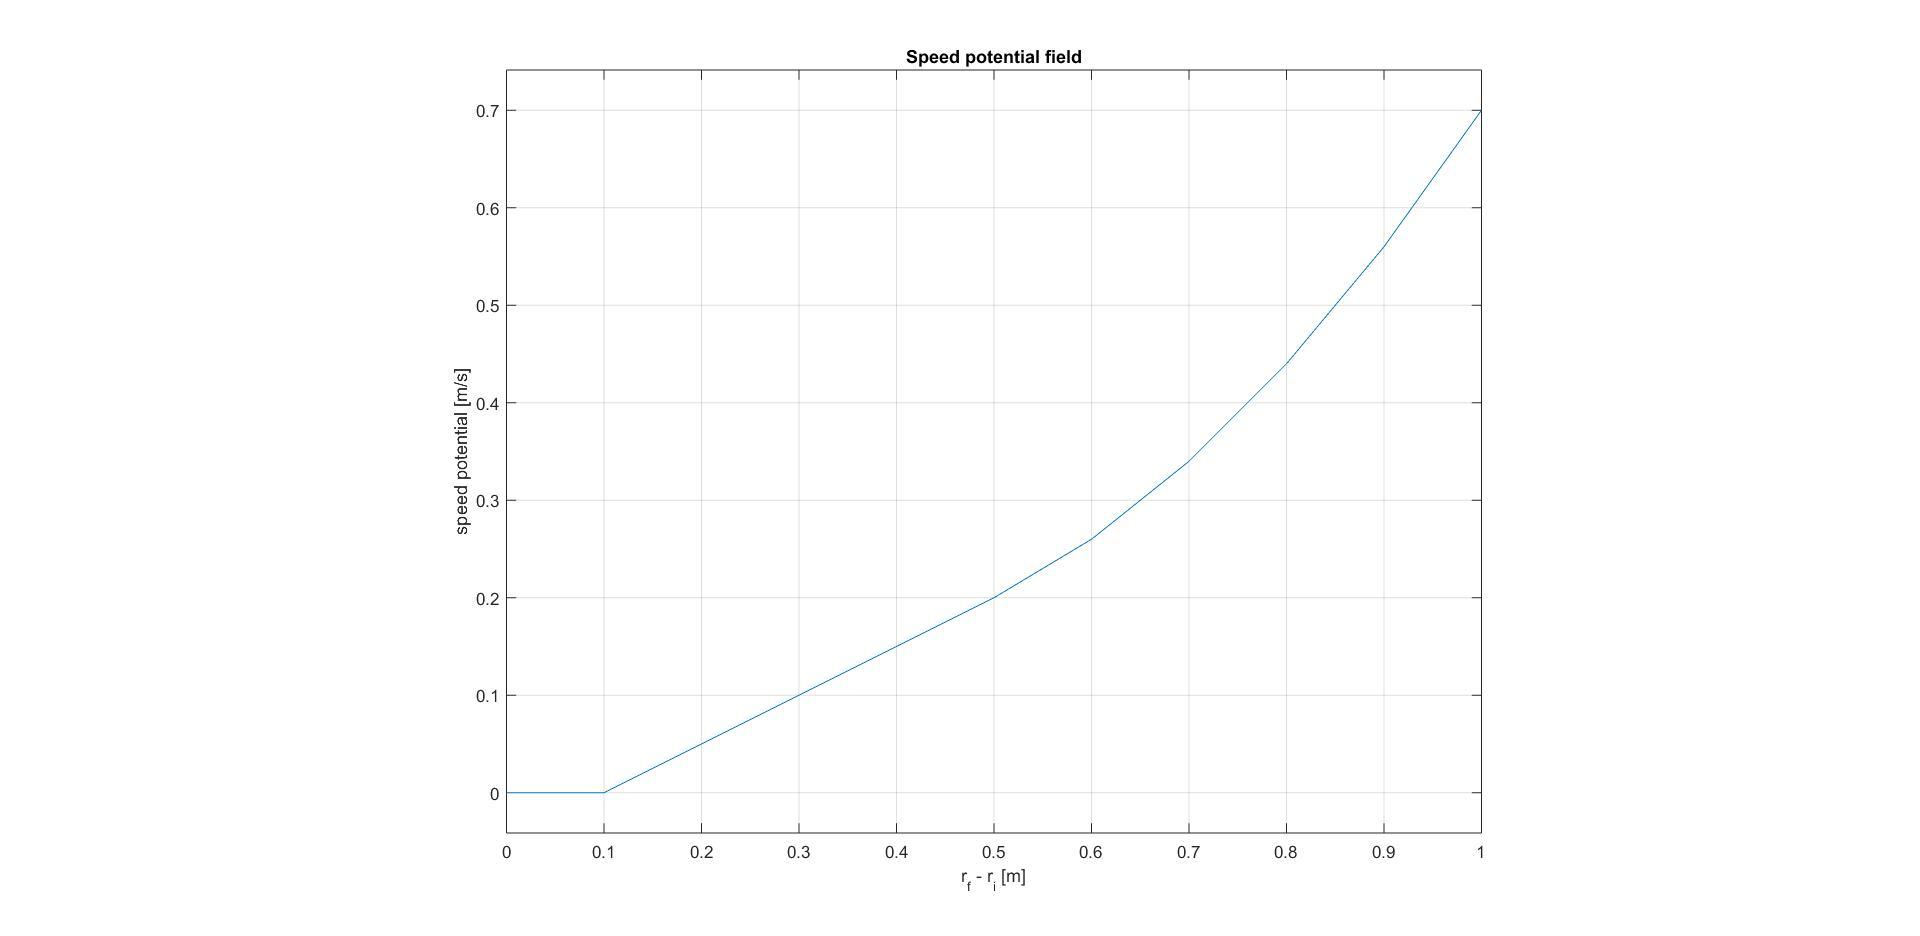
\includegraphics[width=.5\textwidth]{Images/potentialEx}\label{fig:potentialEx}}
\caption{Potential field controllers}
\label{fig:potentialCont}
\end{figure}

Considering, graph-based controllers, only virtual structure formations can be implemented. The controllers are derived from the so-called consensus problems, in which a set of agent with different initial states converge iteratively to a single final state, identical for all agents \cite{Ren2005}. Using notions of graph-theory, a formation can easily be induced (c.f.: figure~\ref{fig:laplacianTraj}). Moreover, while obstacle avoidance can easily be implemented, collision avoidance with others robot cannot (c.f.: figure~\ref{fig:laplacianDist}). Nevertheless, as stated before for virtual structures, remotely controlling the formation can be tough, especially in case of decentralized controller.  In order to derive a controller, the following notions are required:
\begin{itemize}
\item $\mathcal{G} = <\mathcal{N}, \mathcal{E}>$, an (un)directed graph.
\item $\mathcal{N} = \{R_1, \ldots, R_n\}$, the finite nodes set,  with $n$, the number of robots.
\item $\mathcal{E} \in \mathcal{N}^2, \mathcal{E} = \{(Ri,Rj)| R_i, R_j \in \mathcal{N} and\ i \neq j\} = \{e_1, \ldots, e_m\} $, the (un)directed finite edges set.
\item $A \in  \mathbb{R}^{n \times n} $, the adjacency matrix is a symmetric matrix representing the connections between the nodes:
\[a_{ij} =  \left\{ \begin{matrix*}[l] 1 & if\ (R_i, R_j)\ or\ (R_j, R_i) \in \mathcal{E} \\ 0 & else \end{matrix*} \right.\]
\item $D \in  \mathbb{R}^{n \times n} $, the degree matrix is a symmetric matrix, whose diagonal elements represent the cardinality of each node (i.e.: the sum of edges originating or arriving in this node):
\[d_{ii} =  \sum_{j=1}^{N} a_{ij}\]
\item $B \in  \mathbb{R}^{n \times m} $, the incidence matrix is a matrix, describe which node is connected using which edge. In undirected graphs, edge are given a random direction.
\[b_{ij} =  \left\{ \begin{matrix*}[l] 1 & if\ e_j = (R_i, \bullet) \\-1 & if\ e_j = (\bullet, R_i)  \\ 0 & else \end{matrix*} \right.\]
\item $W \in \mathbb{R}^{m\times m} $, a diagonal weight matrix whose element $w_{i,i}$ corresponds to the weight of edge $e_i \in \mathbb{E}$.
\item $L$ and $L_w\in \mathbb{R}^{n\times n} $, the Laplacian and the weighted Laplacian matrices:
\[ L = D-A = BB^T \qquad L_w = BWB^T\]
\end{itemize}  
The Laplacian and the weighted Laplacian matrices benefits from one interesting property: they positive-semidefinite. This implies that all eigenvalues are nonnegative and, furthermore, at least one eigenvalue is equal to zero. Proofs can be found in \cite{Gowal2013}. 

The feedback law, for state $i$ of all nodes in a N-state system is:
\[ \boldsymbol{\dot x_i}(t) = - L\boldsymbol{x_i}(t)\ for\ i=1, \ldots, N \]
\[\boldsymbol{x_i}(t) \in \mathbb{R}^n\]

The discrete equivalent of the Laplacian feedback control matrix, $L_k \in \mathbb{R}^{n \times n}$, is the stochastic weight of links matrix \cite{Moreau2005}. In a stochastic matrix, the sum of every row is equal to one. Therefore, 1 is an eigenvalue and $\boldsymbol{1}_n$ is the corresponding eigenvector.
\[l_{ij} =  \left\{ \begin{matrix*}[l] \omega_{ij} > 0 & if\  = (R_i, R_j) \in \mathbb{E}\ or\ i=j\\ 0 & else \end{matrix*} \right.\]

\begin{figure}[htbp]
\centering
\subfloat[Formation control with Laplacian feedback]{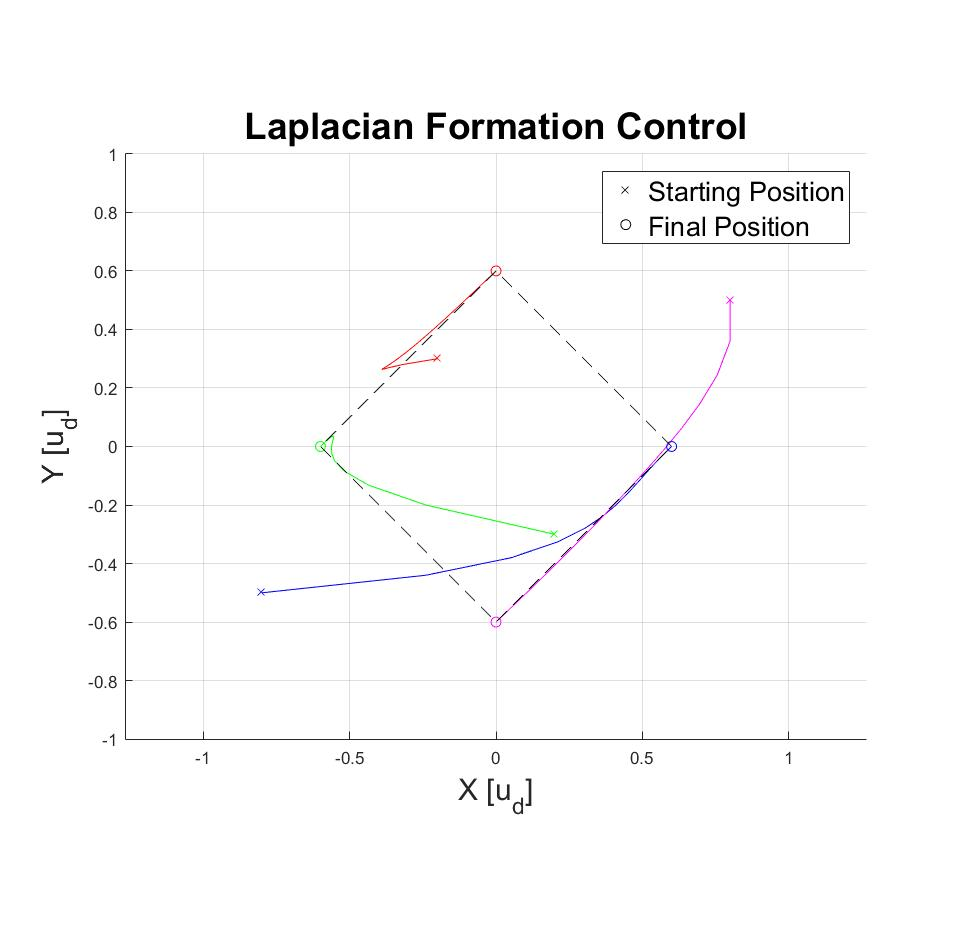
\includegraphics[width=.5\textwidth]{Images/laplacianTraj}\label{fig:laplacianTraj}}
\subfloat[Minimal inter-robot distance. Collision cannot be avoided]{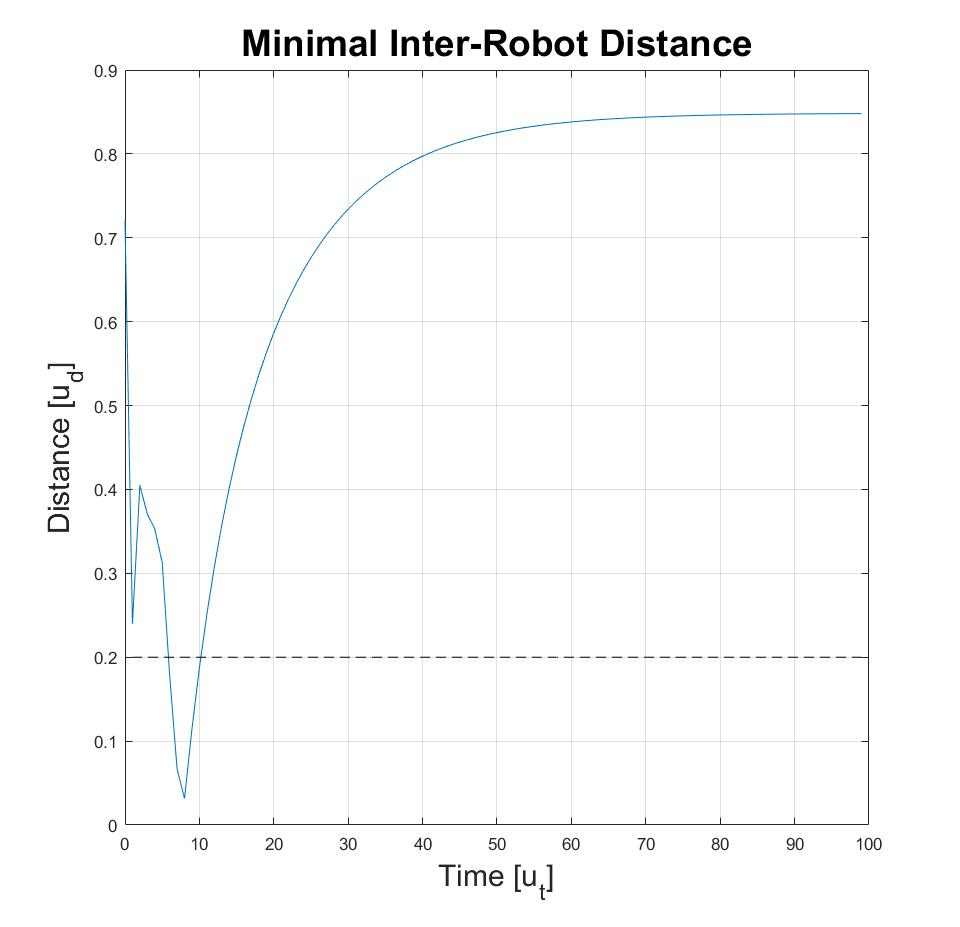
\includegraphics[width=.5\textwidth]{Images/laplacianDist}\label{fig:laplacianDist}}
\caption{Graph-based controllers}
\label{fig:laplacianCont}
\end{figure}

\subsection{Model Predictive Controller}

The outer position controller is part of the model predictive controller, or receding horizon controller, family. This type of nonlinear controllers are especially well suited for constrained application, strongly nonlinear systems or, as the name implies, when future knowledge is desirable \cite{Borelli2015}. In a standard implementation, the controller plans a series of $N$ discrete actions for the open-loop problem, corresponding to the following $N$ time steps by solving a constrained optimization problem. $N$ is referred to as the horizon length. And the longer the horizon length, the closer the open-loop prediction (the $N$ planned actions) from the actual closed-loop trajectory. Because the model of the plant is often inaccurate, or because the environment is evolving, the optimization process is repeated every time-step, after executing only the first of the $N$ planned input actions. This series of planning, acting once, measuring, re-planning actions closes the control loop. Despite it's power and its numerous abilities, MPC suffers from a very high computational cost compared to traditional control methods. Moreover, guaranteeing stability, robustness and feasibility and optimality is a constant trade-off problem.

A MPC controller is the sum of three components: an objective, or cost, function $J$, a set of state dynamics equations and a set of constraints. It can be either derived in continuous or discrete form.

\begin{tabular}{l l l}
\begin{tabular}{r l r l} $J(\boldsymbol{x}, \boldsymbol{u}, t) =$ 	& $V(\boldsymbol{x}(t+T))$  \\ 	& $+\int\limits_t^{t+T} \mathcal{L}(\boldsymbol{x}(t), \boldsymbol{u}(t)dt$  \end{tabular}   & \hspace{.7cm} \vspace{.5cm} & \begin{tabular}{r l r l} $J_k(\boldsymbol{x}, \boldsymbol{u}, t) =$ & $V_k(\boldsymbol{x}(t+NT_s))$  \\  & $+\sum\limits_{k=0}^{N-1} \mathcal{L}_k(\boldsymbol{x}(t+kT_s), \boldsymbol{u}(t+kT_s))$  \end{tabular} \\
$\boldsymbol{\dot x} = f(\boldsymbol{x}, \boldsymbol{u})$ & & $\boldsymbol{x}(k+1) = f_k(\boldsymbol{x}(k), \boldsymbol{u}(k))$ \\
$\boldsymbol{x} \in \mathcal{X}$ and $\boldsymbol{u} \in \mathcal{U}$ & & $\boldsymbol{x} \in \mathcal{X}$ and $\boldsymbol{u} \in \mathcal{U}$ 
\end{tabular}

\subsubsection{Optimization}
Most of the complexity and the cost of using MPC is in solving, at each step, an optimization problem. Therefore, in its first days, MPC was applied to slow systems, with sampling time in minutes or more, especially in the chemical industry. But, its ability to manage constraints made it attractive for other, and faster, applications. Nowadays, thanks to the advance in computers and to efficient numerical algorithms, MPC has been successfully applied to $\mu$s-systems. Nonetheless, to perform control at this rate, trade-offs are made in terms of model complexity, constraint handling and optimality of the control. 

Providing an exhaustive list of solvers for nonlinear constrained optimization is not possible. Nevertheless a rough tentative of classification tempted and a few examples are provided. The first main axis of classification of solvers, and the one that seems recurrent across all literature, is offline (explicit MPC) versus online computing. 

Offline computing consists in explicitly computing the control law for each state (or region of active constraints) and to store it in a table. Most of the computational burden is therefore moved to efficiently search the look-up table for a solution. But, as soon as the number of states, constraints or horizon length increase, the storage requirements increase as well, and exponentially. Therefore, despite being among the fastest algorithms, these methods are limited to small-scale problems \cite{Haverbeke2011}. However Partial Enumeration has been able to tackle large problems for which typical offline and online algorithms are not performing well enough. Although, the solution is not completely computed offline, a subset composed of the most frequent states are. The algorithm stores solutions for the most frequently encountered active sets of constraints and perform online table search. When the solution is not available in the table, several methods exist to compute a sub-optimal but acceptable solution online. The table is constantly kept updated to store only the most recurring sets of active constraints. The main disadvantage of this method is its limitation to QP problems \cite{Pannocchia2007}. 

On the other side, online methods have to solve the optimization problem in every cycle. Surprisingly no commonly accepted categorization has been found. Maybe because of the enormous quantity of problems (QP, LP, least-squares,...) and the huge, already available number of efficient solvers. Especially concerning nonlinear optimization, each author seems to use its own defined terminology. Nonetheless, despite different names, some categories seems to be recurrent across the literature. The main axes of classification are mainly the problem structure (LP, QP, nonlinear) and local versus global search \cite{Haverbeke2011, Nocedal1999, Zheng2015}. Although these categories are not  In what follows, a non-exhaustive presentation of different solving methods are presented.

\begin{itemize}
\item \emph{Gradient methods}: It is certainly the most common type of algorithms to solve linear and nonlinear problems. The main principle is, first an unconstrained version of the problem, to search for a step direction and then move along this direction until the appropriate step size. Iteratively, a travel through improving solution is made until a local minimum is reached. While iterative process can be time consuming, for special kind of problems, a (good) solution can be obtained efficiently or even analytically. It is the case for convex problem formulations such as LP or QP for which many real-time algorithm are available. \cite{Nocedal1999, Wang2008}. Nevertheless, for nonlinear problems, the problem structure cannot be exploited anymore and further refinement have to be made.
\item \emph{Genetic algorithm}: GA are bio-inspired method based on the evolution process. In summary, a population of possible solution is evaluated given a fitness function. The fittest representatives are selected and allowed to generate offspring through linear and nonlinear combinations on one or several of their genotype. The process is repeated until a stop criterion is reached. GA are well-suited for nonconvex and or nonlinear objective functions as many solutions are evaluated and the probability of being stuck in a local minimum is low. Nevertheless, evaluating several individual solutions over several generations is time-consuming. \cite{Zheng2015}
\item \emph{Fuzzy Methods}: In Fuzzy MPC the state space is divided, following a rule-based procedure. Depending on the current state, different LQP representation of the model are used. However, depending on the granularity of the state space rules, offline pre-computation can require a non-negligible storage. Despite the linear models and constraints, these controllers seems to achieve good performance for nonlinear problems. But they currently lack of proven applications and performances.\cite{Zheng2015}.
\end{itemize}


For fast NMPC, two choices are then possible, offline or gradient method. Due to the number of states and constraints to consider, the final choice was made to use the latter. Once again we can part this group in two categories. Sequential Quadratic Programming and Interior Point Methods. The second denomination comprises penalty (including barrier) and more generally augmented Lagrangian methods (or methods of multipliers). With these methods, the goal is, usually to transform the current constrained problem into an unconstrained (or equality constrained one) on which nonlinear gradient method can be applied. In SQP, at each step, the cost function and the constraints are linearized to produce an LQP problem which can be efficiently solved using traditional methods.

Barrier methods, using a logarithmic penalty function, has a neat advantage on the others when it come to LP or QP as it can exploit the typical structure of the problem. However in nonlinear case, it is often less performing than the two others. Both ot these methods has its strength and weaknesses. Augmented Lagrangian requires less mathematical assumptions on the cost and constraints functions, which makes it more general. Moreover they benefit from the simpler framework of unconstrained optimization. On the other hand, SQP usually requires fewer iterations but has to solve a more complex subproblem, which is linearization. \cite{Bertsekas1999, Ruszczynski2006, Nocedal1999, Haverbeke2011,Zheng2015, Tenny2002}

Before the final choice, a quick recall on nonlinear constrained optimization.
The Karush–Kuhn–Tucker conditions have to be derived and solved. Note that the KKT are first order necessary conditions for optimality, therefore they only ensure local optimum. Let us consider a general nonlinear problem:
\[ \min\limits_{\boldsymbol{x}} f(\boldsymbol{x}) \]
\[ s.t \quad h_i(\boldsymbol{x}) = 0 \quad i =1, ..., k \]
\[\quad f_j(\boldsymbol{x}) \leq 0 \quad j =1, ..., l \]

The KKT says that for a (local) optimum solution $\boldsymbol{x}^*$, there exist unique multipliers vectors $\boldsymbol{\lambda}^*$ and $\boldsymbol{\mu}^*$such that:
\[ L(\boldsymbol{x},\boldsymbol{\lambda},\boldsymbol{\mu}) := f(\boldsymbol{x}) + \sum_{i=1}^k h_i\lambda_i  + \sum_{j=1}^l f_j\mu_i \]
\[ \nabla_x L(\boldsymbol{x}^*,\boldsymbol{\lambda}^*,\boldsymbol{\mu}^*) =  \boldsymbol{0} \]
\[h_i(\boldsymbol{x}^*) = 0 \quad i =1, ..., k \]
\[f_j(\boldsymbol{x}^*) \leq 0 \quad j =1 ,..., l \] 
\[ \boldsymbol{\mu}^* \geq  \boldsymbol{0}  \]
\[f_j(\boldsymbol{x}^*) \mu_j^* = 0 \quad j =1, ..., l \]

One of the main difference between IP methods and SQP is the interpretation of the last three constraints. In the latter, they are applied to the linearized system and, in the former,  because the inequality constraints are included in the cost functions, the KKT conditions become \cite{Haverbeke2011}:
\[ \nabla_x L(\boldsymbol{x}^*,\boldsymbol{\lambda}^*,\boldsymbol{\mu}^*) =  \boldsymbol{0} \]
\[h_i(\boldsymbol{x}^*) = 0 \quad i =1, ..., k \]
\[f_j(\boldsymbol{x}^*) \mu_j^* = \tau \quad j =1, ..., l \]
With $\tau$ a parameter depending of the penalty function used.

As seen above, time required to solve the optimization, even if the problem is convex, is always relatively high. In NMPC, this solution is not even ensured to be the global optimum even though globalization techniques exist.  Most of the cost, in terms of computational time, is caused by the iterative requirements of gradient methods. Nevertheless, several artifacts can be used to fasten the computation process, for linear and nonlinear problems. First, warm-starting strategies, consisting of providing a good starting point, allows to reduce the number of iteration. More simply, limiting the number of iteration, or premature termination can generate a great gain of time. Although,suboptimal solutions are provided, they are often good enough. Moreover, several methods exist also to determine the step direction: steepest descent, Nesterov fat gradient \cite{Richter2012}, Krylov-subspace \cite{Ohtsuka2004}. Every choice is a trade-off between speed of convergence, storage, robustness, computational cost and more. For QP problems, a strategic variable reordering can make arise a specific matrix structure, which results in a reduced computational cost. \cite{Wang2008}.

Despite, SQP seems to be faster, the choice has been made to use an IP method, the Continuation-Generalized Minimum Residual method.\cite{Ohtsuka2004}. In this method, iterations are extremely limited which make it extremely fast and able to run the controller for the formation control problem. More objectively, both type of methods could have been applied and if the time was allowing it, a comparison would have been made.

More specifically, the C/GMRES method can be assimilated to an augmented Lagrangian method with penalty function for inequalities. Its expression is derived form the Pontryagin maximum principle \cite{Pontryagin1987, Lewis2006, Murray2010}. The maximum principle is a necessary condition of optimal control. A necessary and sufficient one, the Hamilton-Jacobi-Bellman equation, which needs to be satisfied on the whole state space is often intractable.

A general control system is defined as follow, with $\mathcal{X} \subset \mathbb{R}^n$, the state set and $\mathcal{U} \subset \mathbb{R}^m$, the input set.
\[ \Sigma = (\mathcal{X}, f, \mathcal{U}) \]
\[ \Sigma: \boldsymbol{\dot x} = f(\boldsymbol{x}, \boldsymbol{u}),\ \boldsymbol{x} \in \mathcal{X},\ \boldsymbol{u} \in \mathcal{U} \]

In order to minimize an objective function  $J_{\Sigma,\mathcal{L}}$, three necessary conditions can be derived. Nevertheless another mathematical object can be used, the extended Hamiltonian. Note that the the extended Hamiltonian is, in control theory, the equivalent of the augmented Lagrangian. Therefore, it requires also the introduction of the co-state variable (or Lagrange multipliers) $\boldsymbol{\lambda}$:
\[ J_{\Sigma,\mathcal{L}}: \mathcal{X} \times \mathcal{U} \times \mathbb{R_+} \rightarrow \mathbb{R} \]
\[ J_{\Sigma,\mathcal{L}}(\boldsymbol{x}, \boldsymbol{u}, t) = \int_{t}^{t+T} \mathcal{L}(\boldsymbol{x}(t), \boldsymbol{u}(t))dt, \ (\boldsymbol{x}(t), \boldsymbol{u}(t)) \in  \mathcal{X} \times \bar{\mathcal{U}}\]
\[ \mathcal{H}_{\Sigma,\mathcal{L}}: \mathcal{X} \times \mathcal{U} \times \mathbb{R}^n \rightarrow \mathbb{R} \]
\[ \mathcal{H}_{\Sigma,\mathcal{L}}(\boldsymbol{x}, \boldsymbol{u}, \boldsymbol{\lambda}) = \boldsymbol{\lambda}^Tf(\boldsymbol{x}, \boldsymbol{u}) + \mathcal{L}(\boldsymbol{x}, \boldsymbol{u}) \]
To simplify the equations and lighten notation, the extended Hamiltonian $\mathcal{H}_{\Sigma,\mathcal{L}}$ will simply be called Hamiltonian and noted $\mathcal{H}$. As well as $J_{\Sigma,\mathcal{L}}$ will be noted $J$.

The maximum principle states that, for an optimal trajectory $(\boldsymbol{x}^*, \boldsymbol{u}^*)$ for cost function:
\[ J(\boldsymbol{x}, \boldsymbol{u}, t) = V(\boldsymbol{x}(t+T))  + \int_t^{t+T} \mathcal{L}(\boldsymbol{x}, \boldsymbol{u})dt\]
\[ V: \mathcal{X} \rightarrow \mathbb{R} \]
With $ V(\boldsymbol{x}(t+T))$, the terminal cost. Subject to:
\[ \boldsymbol{\dot x} = f(\boldsymbol{x}, \boldsymbol{u}) \]
\[ h_i(\boldsymbol{x}) = 0,\ i = 1, \ldots, k \]
With $h_i(\boldsymbol{x})$, equality state constraints. These constraints can also be adjoined to the Hamiltonian, using another vector of co-state variables $\boldsymbol{\lambda}_h$:
\[ \mathcal{H}_{\Sigma,\mathcal{L}}(\boldsymbol{x}, \boldsymbol{u}, \boldsymbol{\lambda}, \boldsymbol{v}) = \mathcal{L}(\boldsymbol{x}, \boldsymbol{u}) + \boldsymbol{\lambda}^T f(\boldsymbol{x}, \boldsymbol{u}) + \boldsymbol{\lambda}_h^Th(\boldsymbol{x}),\ \boldsymbol{\lambda}_h \in \mathbb{R}^k \]

In the following, $A_b$ denotes either the gradient of a scalar field or the Jacobian of a vector function $A$ with respect to $\boldsymbol{b}$.
\[ A_b = \nabla_b A = \left [ \frac{\partial \mathcal{A}}{\partial b_1} \ldots \frac{\partial \mathcal{A}}{\partial b_n} \right ] \]
\[ A_b =  \begin{bmatrix} \frac{\partial A_1}{\partial b_1} & \frac{\partial A_1}{\partial b_2} & \cdots & \frac{\partial A_1}{\partial b_s}  \\ 
 \frac{\partial A_2}{\partial b_1} &  \frac{\partial A_2}{\partial b_2} & \cdots & \frac{\partial A_2}{\partial b_s}  \\ 
 \vdots &  \vdots & \ddots & \vdots  \\ 
 \frac{\partial A_r}{\partial b_1} &  \frac{\partial A_r}{\partial b_2} & \cdots & \frac{\partial A_r}{\partial b_s} \end{bmatrix}  \]
 
There exist $\boldsymbol{\lambda}^*$ and $\boldsymbol{\lambda}_h^*$ such that:
\[ \boldsymbol{\dot x}^* = \mathcal{H}_\lambda^T (\boldsymbol{x}^*, \boldsymbol{u}^*, \boldsymbol{\lambda}^*, \boldsymbol{\lambda}_h^*)  \qquad \boldsymbol{\dot \lambda}^*  = -\mathcal{H}_x^T (\boldsymbol{x}^*, \boldsymbol{\mu}^*, \boldsymbol{\lambda}^*, \boldsymbol{\lambda}_h^*)\]
\[ \boldsymbol{\lambda}(t+T)^* = V_x^T(\boldsymbol{x}^*(t+T)) \]
And:
\[ H(\boldsymbol{x}^*, \boldsymbol{\mu}^*, \boldsymbol{\lambda}^*, \boldsymbol{\lambda}_h^*) \leq H(\boldsymbol{x}^*, \boldsymbol{u}, \boldsymbol{\lambda}^*, \boldsymbol{\lambda}_h^*) \forall \boldsymbol{u} \in \mathcal{U} \]
Additionally, if the input are unconstrained (i.e.: $\mathcal{U}=\mathbb{R}^m$), a necessary condition for optimal input sequence is:
\[ \mathcal{H}_u (\boldsymbol{x}, \boldsymbol{u}, \boldsymbol{\lambda}, \boldsymbol{\lambda}_h) = \boldsymbol{0}_m \]
  
This last characteristic is part of the foundations of the C/GMRES method. Therefore, instead of constraining the input set, a penalty function is incorporated in the Lagrangian such that $\mathcal{U}=\mathbb{R}^m$. Another exploited characteristic in the method, more globally related to nonlinear optimization, is that the optimal trajectory varies smoothly with respect to time. This part of the algorithm is what is called the continuation, or homotopy, method. It is strategically combined with GMRES in order to quickly solve large linear equations. The main idea of C/GMRES is to compute the derivative of the input sequence and to integrate it other time, instead of computing at each step a new input sequence.

Starting from an approximated version of the optimization problem using forward discretization. For simplification,a mapping from $[t; t+T]$ to $[0; T]$ is performed and $\boldsymbol{x}(t = kT_s)$ is denoted $\boldsymbol{x}(k)$ with $T_s$ the sampling time.
\[ J_k = V(\boldsymbol{x}(N)) + \sum_{k = 0}^{N-1} \mathcal{L}(\boldsymbol{x}(k), \boldsymbol{u}(k))T_s \]
Subject to:
\[ \boldsymbol{x}(k+1) = \boldsymbol{x}(k) + f(\boldsymbol{x}(k),\boldsymbol{u}(k))T_s \]
\[ \psi_i(\boldsymbol{x}(k)) = 0,\ i = 1, \ldots, q_k \]

Then a discretized version of the Pontryagin principle for unconstrained input can be written:
\[ \mathcal{H}_u(\boldsymbol{x}^*, \boldsymbol{u}^*, \boldsymbol{\lambda}^*, \boldsymbol{\lambda}_h^*) = \boldsymbol{0}_m \]
\[ \boldsymbol{\lambda}^*(k)  = \boldsymbol{\lambda}_i^*(k+1) + \mathcal{H}_x^T(\boldsymbol{x}^*, \boldsymbol{u}^*, \boldsymbol{\lambda}^*, \boldsymbol{\lambda}_h^*) T_s\]
\[ \boldsymbol{\lambda}^*(N) = V_x^T(\boldsymbol{x}^*(N)) \]
The control input $\boldsymbol{u}^*$ and the multipliers $\boldsymbol{\lambda}_h^*$ can be computed solving a set of N(m+q) equations. The vector U is defined as follow:
\[\boldsymbol{U} = [\boldsymbol{u}(0), \boldsymbol{\lambda}_h(0), \boldsymbol{u}(1), \boldsymbol{\lambda}_h(1), \ldots, \boldsymbol{u}(N-1), \boldsymbol{\lambda}_h(N-1)]^T \]
\[F(\boldsymbol{U},\boldsymbol{x}) := \begin{bmatrix} \mathcal{H}_u^T(\boldsymbol{x}(0), \boldsymbol{u}(0), \boldsymbol{\lambda}(1), \boldsymbol{\lambda}_h(0)) \\ \boldsymbol{\psi}(\boldsymbol{x}(0)) \\ \vdots \\ \mathcal{H}^T_u (\boldsymbol{x}(N-1), \boldsymbol{u}(N-1), \boldsymbol{\lambda}(N), \boldsymbol{\lambda}_h(N-1)) \\ \boldsymbol{\psi}(\boldsymbol{x}(N-1))\end{bmatrix} = \boldsymbol{0}_{N(m+q)}\]

To simplify notation, $F = F(\boldsymbol{U},\boldsymbol{x})$. Continuation method consists of, starting with a solution of a known problem, for example $F = 0$ at time $t$, computing the solution of another problem, about which few knowledge concerning solutions is known, for example $F = 0$ at time $t + T_s$ \cite{Allgower1987}. Applied to the controller, it means that the equations $F = \boldsymbol{0}_{N(m+q)}$ are not computed every sampling time. Instead $\boldsymbol{\dot U}$ is computed such that:
\[ F(\boldsymbol{U} + \boldsymbol{\dot U}T_s,\boldsymbol{x} + \boldsymbol{\dot x} T_s) = \boldsymbol{0}_{N(m+q)} \]
\[ \boldsymbol{\dot U} = F_U^{-1}(A_s F - F_x \boldsymbol{\dot x}) \]
$A_s$ is a matrix whose role is to stabilize $F = \boldsymbol{0}_{N(m+q)}$ under certain conditions and $F_u$ is required to be nonsingular. A noticeable constraint of this method is the requirement to solve the system $F=0$ at least once at $t=0$.

In order to reduce the cost of solving the linear equations, two additional tools are used, forward difference approximation for Jacobian and vector products, and the GMRES method for solving linear equations.
The product approximation is computed as follow:
\[ F_U(\boldsymbol{U}, \boldsymbol{x}) \boldsymbol{W} + F_x(\boldsymbol{U}, \boldsymbol{x}) \boldsymbol{w} \approx D_h F(\boldsymbol{U}, \boldsymbol{x} : \boldsymbol{W}, \boldsymbol{w}) := \frac{F(\boldsymbol{U} + h\boldsymbol{W}, \boldsymbol{x} + h\boldsymbol{w}) - F(\boldsymbol{U}, \boldsymbol{x})}{h} \]

Then the linear equation to solve becomes:
\[ D_h F(\boldsymbol{U}, \boldsymbol{x}+ h\boldsymbol{\dot x} : \boldsymbol{\dot U}, 0) = A_s F(\boldsymbol{U}, \boldsymbol{x}) - D_h F(\boldsymbol{U}, \boldsymbol{x} : 0, \boldsymbol{\dot x}) := \boldsymbol{b}(\boldsymbol{U}, \boldsymbol{x}, \boldsymbol{\dot x}) \]

The GMRES tool (or Forward Difference GMRES, FDGMRES, in \cite{Kelley1995}) is an iterative Krylov subspace method to solve linear systems of equations. It can be decomposed in three steps.

First, the initialization of the residual $\hat r$ and the Krylov basis $\mathcal{V}_\mathcal{K}$ with an initial guess $\boldsymbol{\hat{ \dot U}}$ on the control input derivative:
\[ \boldsymbol{\hat r} := \boldsymbol{b}(\boldsymbol{U}, \boldsymbol{x}, \boldsymbol{\dot x}) - D_h F(\boldsymbol{U}, \boldsymbol{x}+ h\boldsymbol{\dot x} : \boldsymbol{\hat{\dot U}}, 0) \]
\[\boldsymbol{v_1} := \frac{\boldsymbol{\hat r}}{\norm{\boldsymbol{\hat r}}},\ \rho = \norm{\boldsymbol{\hat r}},\ \beta: = \rho \].

Then, the loop iteration while $k_{loop} < k_{loop,max}$:
\begin{enumerate}
\item $k = k+1$
\item Compute a new basis vector for $\mathcal{V}_\mathcal{K}$: $\boldsymbol{v}_{k+1} =  D_h F(\boldsymbol{U}, \boldsymbol{x}+ h\boldsymbol{\dot x} : \boldsymbol{v_k}, 0)$.
\item Normalization, orthogonalization using Gramm-Schmidt process and construction of matrix $H_k$:
\[ Loop: h_{j,k} = \boldsymbol{v}_{k+1}^T \boldsymbol{v}_j,\ \boldsymbol{v}_{k+1} = \boldsymbol{v}_{k+1} - h_{j,k}\boldsymbol{v}_j, \quad for\ j = 1, \ldots, k \]
\[ h_{k+1,k} = \norm{\boldsymbol{v}_{k+1}} \]
\[ h_{k+1, j} =  0\quad for\ j = 1, \ldots, k-1 \]
\[ \boldsymbol{v}_{k+1} = \frac{\boldsymbol{v}_{k+1}}{\norm{\boldsymbol{v}_{k+1}}} \]
\item Solve $\min\limits_{y_k}\norm{\beta \boldsymbol{e}_1 - H_k\boldsymbol{y}_k}$, with $\boldsymbol{y}_k in \mathbb{R}^k$.
\item Residual length $\rho = \norm{\beta \boldsymbol{e_1} - H_k\boldsymbol{y}_k}$.
\end{enumerate}

The minimization step can be solved efficiently using Givens rotations \cite{Bjorck1996}. Which consists of applying consecutive rotations $G_i(\theta_i)$ to the system untill $\prod_i G_i(\theta_i) H_k$ is upper triangular.
A Givens rotation matrix $G(p, q, \theta)$ is defined  as follow:
\[ g_{ij} = \left\{ \begin{matrix*}[l] \cos{\theta} &  if\ i = j = p, q \\ 1 & if\ i = j \neq p, q  \\  -\sin{\theta} &  if\ i = p,\ j = q \\ \sin{\theta} &  if\ i = q,\ j = p \\ 0 & else \end{matrix*} \right.\]
In the code, at iteration $k$, the matrix $G_k$ is computed:
\[ G_k := G_k(k, k+1, \theta_k) \quad with\ \theta_k = atan2(h_{k+1, k}, h_{k,k})\]
Which result in:
\[ \min\limits_{y_k}(\norm{\prod\limits_{i=1}^k G_i(i, i+1, \theta_i) (\beta \boldsymbol{e}_1 - H_k \boldsymbol{y}_k)} \]

As an iterative process, it is typically costly. However, limiting the number of iterations to $k_{max}$, keep its influence small on the whole algorithm duration but produces in a suboptimal solution.

The final step is the computation of solution:
\[ \boldsymbol{\dot U} = \boldsymbol{\hat{ \dot U}} + V_k \boldsymbol{y}_k \]
With $V_k = [v_1, \ldots, v_k]$ the Krylov subspace basis $\mathcal{V}_\mathcal{K}$.

Now, continuation and GMRES method can be combined to produce C/GMRES:
\begin{enumerate}
\item Initialization: compute $\boldsymbol{U}(0)$ numerically or anatically.
\item Loop over k:
\begin{enumerate}
\item Apply first input of sequence: $\boldsymbol{u}(k) = \boldsymbol{U}_{1:m}(k)$.
\item Measure $\boldsymbol{x}(k)$, Compute $\Delta x = \boldsymbol{x}(k) - \boldsymbol{x}(k-1)$.
\item Compute $\boldsymbol{\dot U}(k)$ using GMRES with $\dot x = \frac{\Delta x}{Ts}$ and $\boldsymbol{\hat{\dot U}}(k) = [\boldsymbol{\dot U}^T_{m+q+1:N(m+q)}(k-1)\ \boldsymbol{0}_{m+q}]^T $ (i.e.: the input of last time step, without the first elements corresponding to the input applied and padded with zeros).
\end{enumerate}
\item k = k+1.
\end{enumerate}

\subsubsection{Model}
The model used in the formation controller, is very generic in order to be easily transferable to other flying (or terrestrial or swimming) platforms. It simply consists of the linear second order translational model augmented with heading control. 

It is constantly assumed that the working point around which the drone operate is  the hovering point given by:
\[\boldsymbol{x_s} = \begin{bmatrix}\dot x \\ \dot y \\ \dot z \\ \ddot x \\ \ddot y \\ \ddot z \\ \dot \psi\end{bmatrix} = \begin{bmatrix} 0 \\ 0 \\ 0 \\ 0 \\ 0 \\ 0 \\ 0\end{bmatrix} \quad \boldsymbol{u_s} = \begin{bmatrix} f_x \\ f_y \\ f_z \\ \dot \psi \end{bmatrix} = \begin{bmatrix}  0\\ 0\\ mg \\ 0\end{bmatrix} \]

Then, the model for one drone is:

 \[\boldsymbol{x} =  [x \ y \ z \ \dot x \ \dot y \ \dot z \ \psi]^T \]
\[\boldsymbol{\dot x} =  A \boldsymbol{x} + B \boldsymbol{u} \]
\[\begin{bmatrix}\dot x \\ \dot y \\ \dot z \\ \ddot x \\ \ddot y \\ \ddot z \\ \dot \psi\end{bmatrix}  = 
\begin{bmatrix}  0 & 0 & 0 & 1 & 0 & 0 & 0 \\ 0 & 0 & 0 & 0 & 1 & 0 & 0 \\ 0 & 0 & 0 & 0 & 0 & 1 & 0 \\ 0 & 0 & 0 & 0 & 0 & 0 & 0 \\ 0 & 0 & 0 & 0 & 0 & 0 & 0 \\ 0 & 0 & 0 & 0 & 0 & 0 & 0 \\ 0 & 0 & 0 & 0 & 0 & 0 & 0 \end{bmatrix} 
\begin{bmatrix} x \\ y \\ z \\ \dot x \\ \dot y \\ \dot z \\ \psi \end{bmatrix}  + \begin{bmatrix}  0 & 0 & 0 & 0 \\ 0 & 0 & 0 & 0 \\ 0 & 0 & 0 & 0 \\ \frac{1}{m} & 0 & 0 & 0 \\ 0 & \frac{1}{m} & 0 & 0 \\ 0 & 0 & \frac{1}{m} & 0 \\ 0 & 0 & 0 & 1 \end{bmatrix} \begin{bmatrix} f_x \\ f_y \\ f_z \\ \dot \psi \end{bmatrix} \]

The full model is:
\[\begin{bmatrix}\boldsymbol{\dot x}_1 \\ \boldsymbol{\dot x}_2 \\ \boldsymbol{\dot x}_3 \\ \boldsymbol{\dot x}_4\end{bmatrix}  = 
\begin{bmatrix}  A & 0 & 0 & 0 \\ 0 & A & 0 & 0 \\ 0 & 0 & A & 0 \\ 0 & 0 & 0 & A \end{bmatrix} 
\begin{bmatrix}\boldsymbol{x}_1 \\ \boldsymbol{x}_2 \\ \boldsymbol{x}_3 \\ \boldsymbol{x}_4\end{bmatrix}  + 
\begin{bmatrix}  B & 0 & 0 & 0 \\ 0 & B & 0 & 0 \\ 0 & 0 & B & 0 \\ 0 & 0 & 0 & B \end{bmatrix} 
\begin{bmatrix}\boldsymbol{u}_1 \\ \boldsymbol{u}_2 \\ \boldsymbol{u}_3 \\ \boldsymbol{u}_4\end{bmatrix} \]

The first part of the control input, for each drone, a 3 dimensional forces vector in thrust, roll and pitch command solving:
\[ R_{BW}^T(\phi, \theta, \psi) \begin{bmatrix}  0\\ 0\\ F_z \end{bmatrix}_B = \begin{bmatrix}  f_x\\ f_y\\ f_z \end{bmatrix} = \boldsymbol{u}_{j,1:3} \quad j = 1, \ldots , 4\]
More details about this operations are given in section \ref{sec:ForceToAngle}

%The drag force, in a turbulent air flow, is usually defined as:
%\[ \boldsymbol{D} = -(\frac{1}{2} \norm{\boldsymbol{\dot r}}^2 C_D A) \frac{\boldsymbol{\dot r}}{\\norm{\boldsymbol{\dot r}}}\]
%Where $\boldsymbol{\dot r}$ is the relative speed of the quadcopter to the fluid, $\rho$ is the air density, $C_D$  the drag coefficient and $A$t the cross-sectional area (i.e.: the maximal area of the quadrotor in the plane perpendicular to the speed vector $\boldsymbol{\dot r}$). For modeling purpose, it can be simplified as follow:
%\[ \boldsymbol{D} \approx -K_d(\psi) \norm{\boldsymbol{\dot r}} \boldsymbol{\dot r}\]
%
%\textcolor{red}{A DEVELOPPER}

%The reduced linearized model is:
%
%Finally, the model is discretized, with sampling time $T_s$:
%\[\begin{bmatrix} x_{k+1} \\ y_{k+1} \\ z_{k+1} \\ \dot x_{k+1} \\ \dot y_{k+1} \\ \dot z_{k+1} \\ \psi_{k+1} \end{bmatrix}  = 
%\begin{bmatrix}  1 & 0 & 0 & T_s & 0 & 0 & 0 \\ 0 & 1 & 0 & 0 & T_s & 0 & 0 \\ 0 & 0 & 1 & 0 & 0 & T_s & 0 \\ 0 & 0 & 0 & 1 & 0 & 0 & 0 \\ 0 & 0 & 0 & 0 & 1 & 0 & 0 \\ 0 & 0 & 0 & 0 & 0 & 1 & 0 \\ 0 & 0 & 0 & 0 & 0 & 0 & 1 \end{bmatrix} 
%\begin{bmatrix} x_k \\ y_k \\ z_k \\ \dot x_k \\ \dot y_k \\ \dot z_k \\ \psi_k \end{bmatrix}  + \begin{bmatrix}  \frac{T^2_s}{2m} & 0 & 0 & 0 \\ 0 & \frac{T^2_s}{2m} & 0 & 0 \\ 0 & 0 & \frac{T^2_s}{2m} & 0 \\ \frac{T_s}{m} & 0 & 0 & 0 \\ 0 & \frac{T_s}{m} & 0 & 0 \\ 0 & 0 & \frac{T_s}{m} & 0 \\ 0 & 0 & 0 & T_s \end{bmatrix} \begin{bmatrix} f_{x,k} \\ f_{y,k} \\ f_{z,k} \\ \dot \psi_k \end{bmatrix} \]
\subsubsection{Constraints}
The following constraints were implemented:
\begin{itemize}
\item \emph{collision avoidance}: $ \norm{\boldsymbol{x}_{i,1:3}-\boldsymbol{x}_{j,1:3}}^2 \geq R_r^2, \quad i,j = 1, \ldots, 4, i \neq j$\\
It simply means that the drones have to keep a certain distance between their positions
\item \emph{input constraint}:  $ f_{i,x}^2 + f_{i,y}^2 \leq (mg \cdot \alpha_{max})^2 $. \\
This constraint ensures to stay around the hovering point as well.  Concretely it means that the force in the horizontal plan should not exceed the projection of the gravity force when the drone is moving (c.f.: figure ~\ref{fig:inputConst}). Furthermore as $\alpha_max$ is assumed to be small, small angle approximation is made. One advantage of expressing the constraint in this matter, is that we constraint the combined effect of the pitch and the roll angles instead of  constraining them individually.
\end{itemize}

\begin{figure}[htbp]
\centering
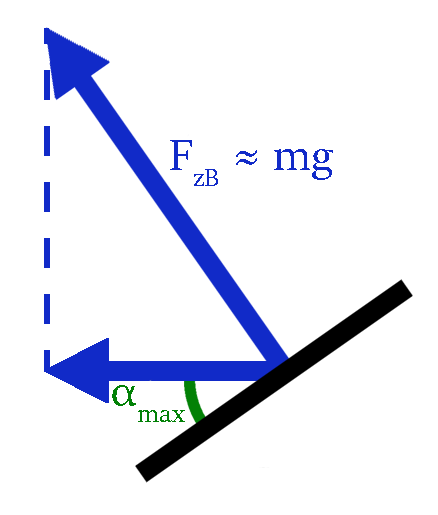
\includegraphics[width=.4\textwidth]{Images/inputConst}
\caption{The input constraint explained}
\label{fig:inputConst}
\end{figure}

\subsubsection{Cost Function}
As said before, the inequalities constraints have to be included in the objective function. It is proposed in \cite{Ohtsuka2004} to use a quadratic penalty function, which is differentiable. Moreover keeping the the place in formation can be considered as a tracking problem in which the reference is unknown. For this, a quadratic cost function is used. Finally, the objective function is:
\[ J(\boldsymbol{x}, \boldsymbol{u}, t) = (\boldsymbol{x}-\boldsymbol{x}_r)^T(t+T)S(\boldsymbol{x}-\boldsymbol{x}_r)(t+T)  + \int_t^{t+T} (\boldsymbol{x}-\boldsymbol{x}_r)^T(t)Q(\boldsymbol{x}-\boldsymbol{x}_r)(t) + \boldsymbol{u}^T(t)R\boldsymbol{u}(t)  \]
\[ + \gamma_r \sum_{i=1}^3 \sum_{j=i+1}^4 \max(0; R_r^2 -  \norm{\boldsymbol{x}_{i,1:3}(t)-\boldsymbol{x}_{j,1:3}(t)}^2)^2 \]
\[+ \gamma_u \sum_{i=1}^4 \max(u_{i,1}^2(t) + u_{i,2}^2(t) - (mg \cdot \alpha_{max})^2)^2 dt \]


\newpage
\section{Low-Level Control - Attitude Control}
\subsection{Attitude Controller}
\label{sec:innerControl}
The inner controller, responsible for attitude control can be found in the stabilizer.c module. Its main loop can be divided in four steps, the corresponding files are indicated in brackets:
\begin{itemize}
\item State acquisition (\emph{sensors\_stock.c} and \emph{estimator\_complementary.c}  or \emph{estimator\_kalman.c}).
\item Reference acquisition (\emph{commander.c}).
\item Control step (\emph{controller\_pid.c} and then \emph{attitude\_pid\_controller.c} and \emph{pid.c}).
\item Motor distribution (\emph{power\_distribution\_stock.c}).
\end{itemize}

\subsubsection{State and Reference Acquisition}
Independently of the chosen estimation method, 13-states Kalman filter or attitude update through Mahony or Magdwick quaternion method, the first step is to estimate the attitude angles and rates. However, the chosen method will have an impact on the estimation and the stabilizer frequency, a Kalman estimator runs at 100 \emph{Hz} and limits at the stabilizer loop 500 \emph{Hz}, while the other method car run at 250 \emph{Hz} and the stabilizer loop can operate 1000 \emph{Hz}. In both cases, sensor acquisition runs at 500 \emph{Hz} for IMU and 100 \emph{Hz} for barometer.

During the acquisition of the references, the inner control architecture is also defined or updated. Depending on the control mode, the reference are translated differently and the chain of controller is activated accordingly. There are six configuration variables, each can be set in absolute, velocity or disabled mode.  These variables are X, Y, Z, the 3D positions and roll, pitch, yaw, the three attitude angles. In this project, the references sent are always roll angle, pitch angle, yaw rate and thrust (c.f.: table~\ref{tab:setpointConfig}). Despite the presence of a magnetometer in the IMU, yaw control is not possible as the estimator has not yet included the sensor data.

\begin{table}[htbp]
\centering
\caption{Reference and inner control architecture configuration}
\begin{tabular}{|l|c|}
\hline
\textbf{Configuration variables} & \textbf{State}  \\
\hhline{|=|=|}
Position X & Disabled \\
\hline
Position Y & Disabled \\
\hline
Position Z & Disabled \\
\hline
Attitude Roll & Absolute\\
\hline
Attitude Pitch & Absolute\\
\hline
Attitude Yaw & Velocity\\
\hline
\end{tabular}
\label{tab:setpointConfig}
\end{table}

\subsubsection{Controllers}
The first module, \emph{controller\_pid.c}, defines the control architecture and the rate of the two sub-control loops: PID at 100 \emph{Hz} for position control or cascade controllers at 500 \emph{Hz} for attitude control. In the latter (\emph{attitude\_pid\_controller.c}), the yaw rate reference is first integrated to obtain a yaw reference angle, then, the first layer of control is given the attitude angles references and estimations. In the second layer, rates are controlled. The output of the attitude controllers serve as rate reference and the gyros measurements as attitude rate measurement (c.f.: figure~\ref{fig:controllerCascade}). This assumption can be considered as true for small angles or first-order approximations. For exact attitude rate computation, refer to the section~ref:{sec:dynamicsEquations}.  In the cascade controller, both layers  are composed of standard PID controllers using an integral limit as shown in figure~\ref{fig:controllerPID}. Note also that the estimation method has an influence on the gains. In table~\ref{tab:controllerInnerGains}, gains are provided for a CrazyFlie 2.0 using the stock (or attitude-only) estimator.

\begin{figure}[htbp]
\centering
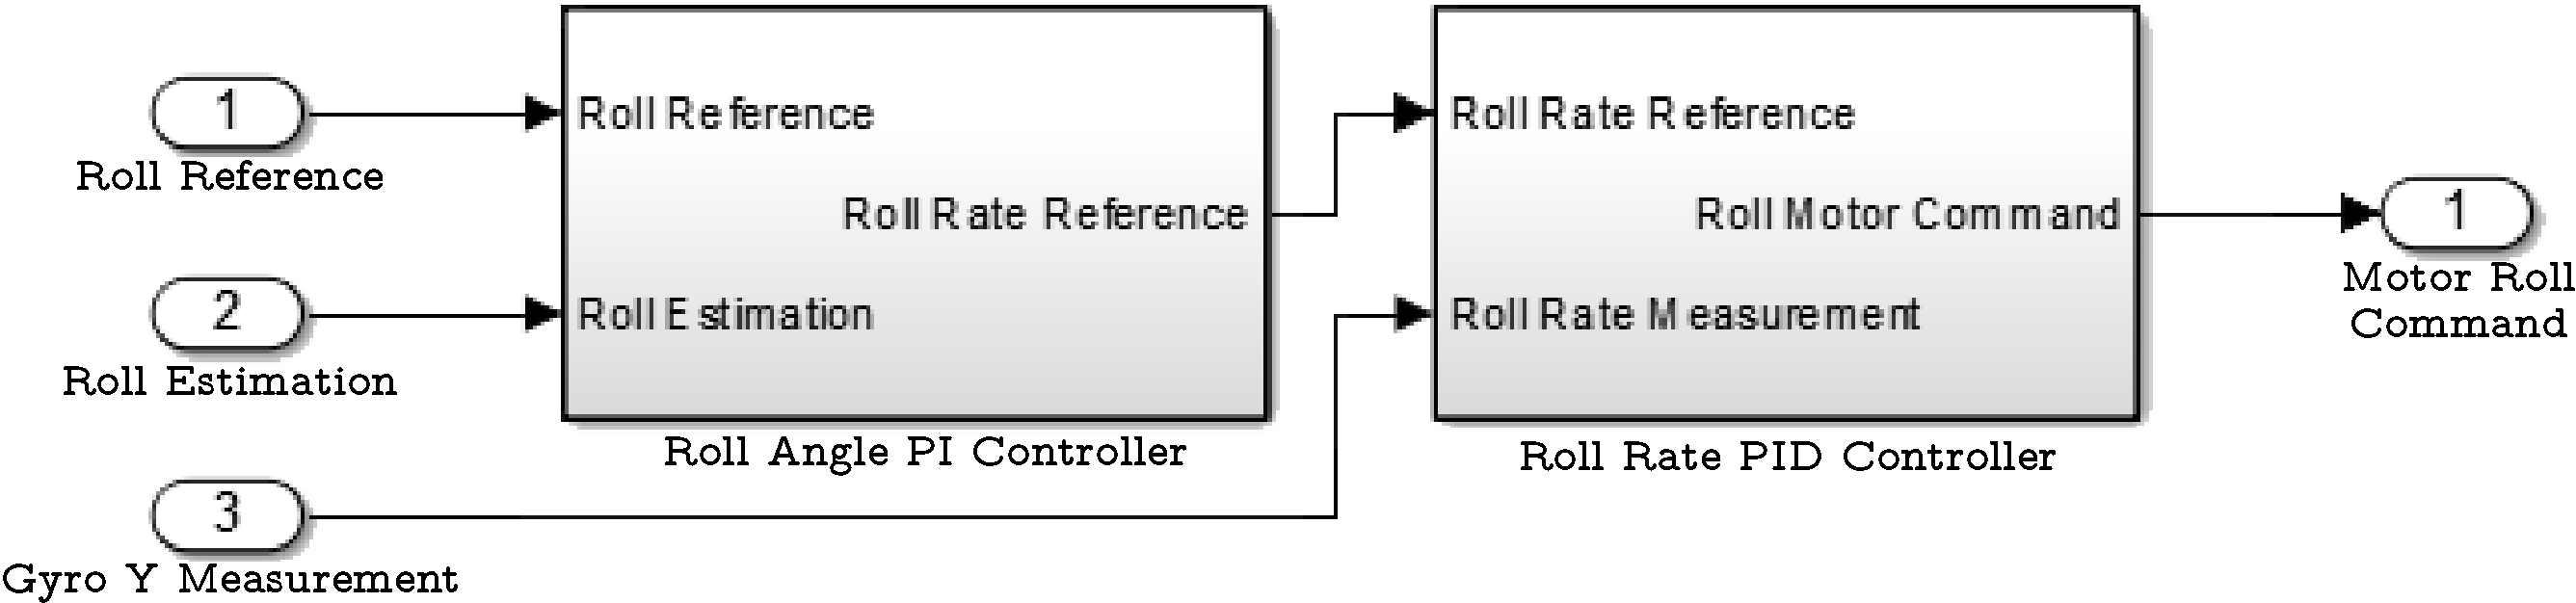
\includegraphics[scale = 0.75]{Images/controllerCascade}
\caption{Roll cascade controller architecture}
\label{fig:controllerCascade}
\end{figure}

\begin{figure}[htbp]
\centering
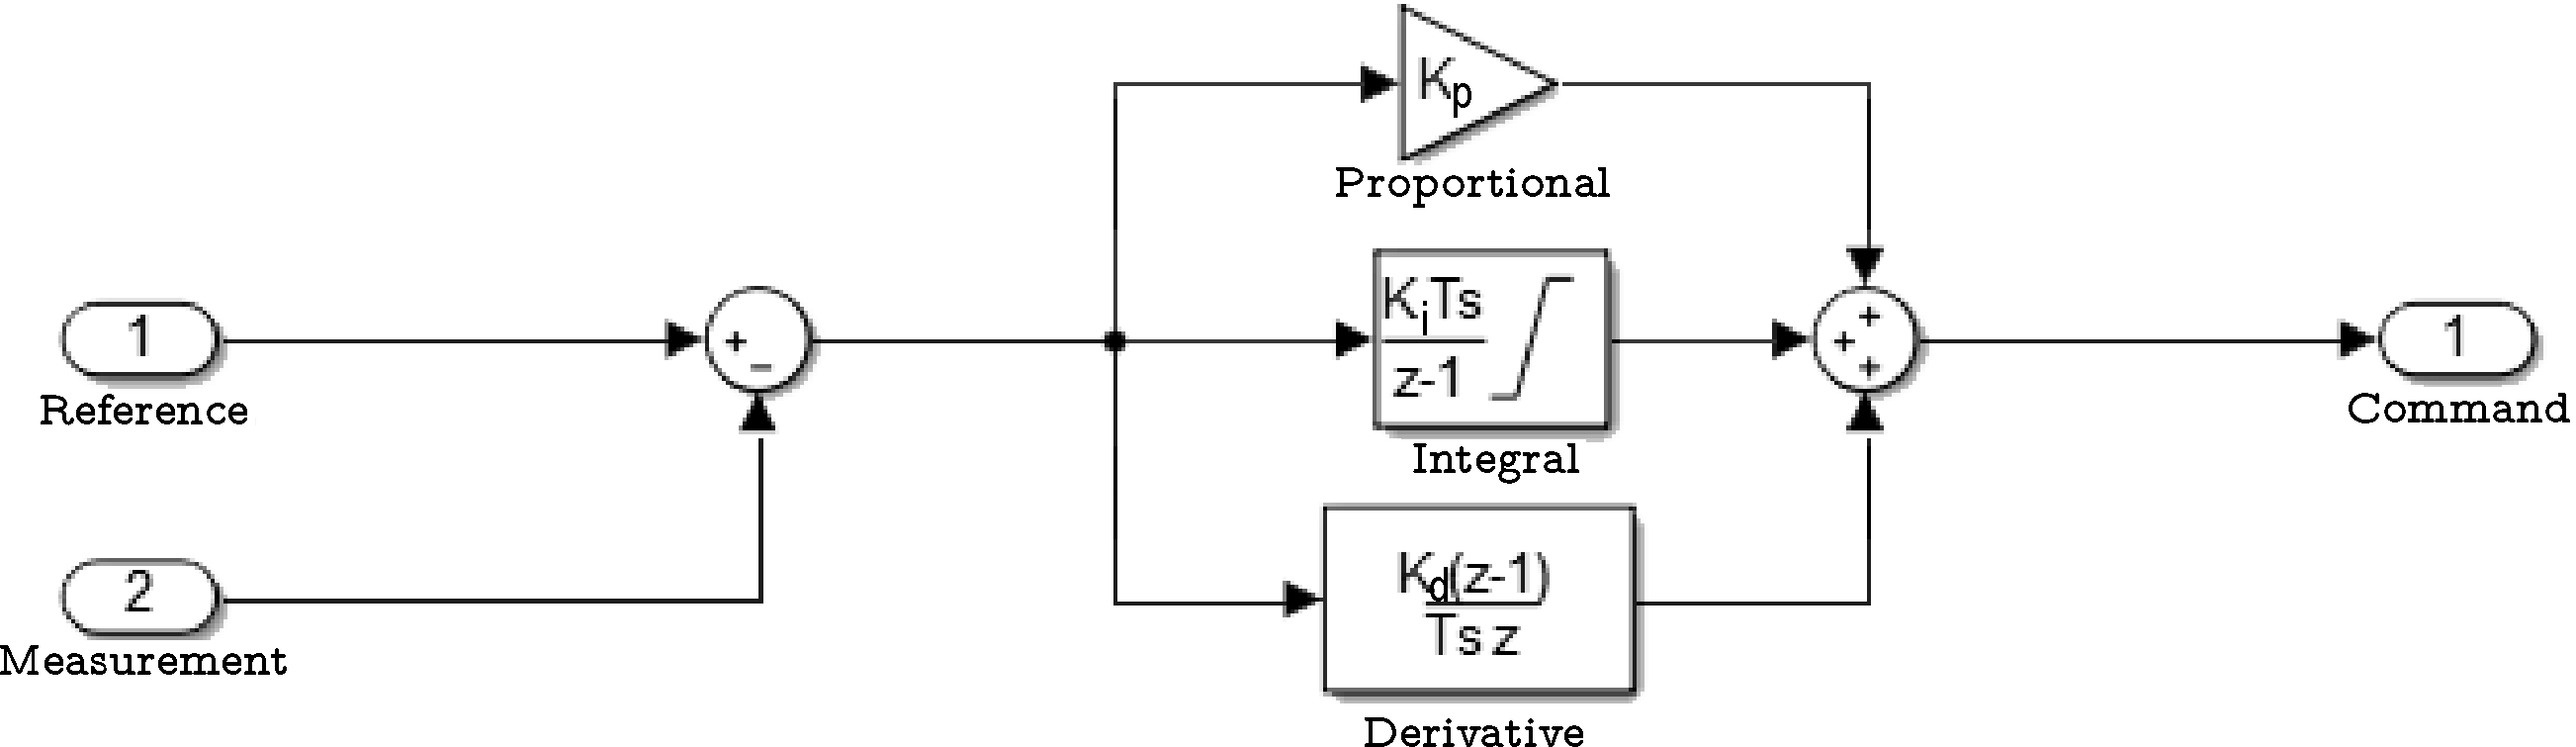
\includegraphics[scale = 0.8]{Images/controllerPID}
\caption{PID controller architecture}
\label{fig:controllerPID}
\end{figure}

\begin{table}[htdp]
\caption{Gains and integral limit of the inner PID controllers}
\centering
\begin{tabular}{|l||c|c|c|c|}
\hline
\textbf{Controller} & $\boldsymbol{K_p}$ & $\boldsymbol{K_i}$ & $\boldsymbol{K_d}$ & \textbf{Integral Limit}  \\
\hhline{|=#=|=|=|=|}
Roll & 6 & 3 & 0 & 20  \\
\hline
Pitch & 6 & 3 & 0 & 20  \\
\hline
Yaw & 6 & 1 & 0.35 & 360  \\
\hline
Roll rate & 250 & 500 & 2.5 & 33.3  \\
\hline
Pitch rate & 250 & 500 & 2.5 & 33.3  \\
\hline
Yaw rate rate & 70 & 16.7 & 0 & 166.7  \\
\hline
\end{tabular}
\label{tab:controllerInnerGains}
\end{table}

\subsubsection{Motor Distribution}
The output of the 3 attitude cascade controllers and the thrust input are combined, with respect to the flying configuration, as shown in table~\ref{tab:motorDistribution}, saturated and converted to a 8-bit PWM value before being transmitted to the motors. 

\begin{table}[htdp]
\caption{Command summation for a $+$  flying configuration}
\centering
\begin{tabular}{|l|l c l c l|}
\hline
\textbf{Motor 1} & $u_{thrust}$ & + &$u_{pitch}$ & + & $u_{yaw}$\\
\hline
\hline
\textbf{Motor 2} & $u_{thrust}$ & - & $u_{roll}$ & - & $u_{yaw}$ \\
\hline
\hline
\textbf{Motor 3} & $u_{thrust}$ & - & $u_{pitch}$ & + & $u_{yaw}$\\
\hline
\hline
\textbf{Motor 4} & $u_{thrust}$ & + & $u_{roll}$ & - & $u_{yaw}$ \\
\hline
\end{tabular}
\label{tab:motorDistribution}
\end{table}

\subsection{Force to Angle and Thrust Commands}
\label{sec:ForceToAngle}
For one quadrotor, we have to solve the following nonlinear system of equations to translate the force vector into an appropriate command:
\[ R_{BW}(\phi, \theta, \psi) \begin{bmatrix}  f_x\\ f_y\\ f_z \end{bmatrix} = \begin{bmatrix}  0\\ 0\\ F_z \end{bmatrix}_B\]

Recall that, the yaw angle $\psi$ is known and:
\[R_{BW}(\phi, \theta, \psi)= R_{Ox}(\phi) R_{Oy}(\theta) R_{Oz}(\psi) \]
Then, we can apply the yaw rotation on the force vector (symbolized as $f'$) and solve:
\[ R_{Ox}(\phi) R_{Oy}(\theta) \begin{bmatrix}  f'_x\\ f'_y\\ f'_z \end{bmatrix} = \begin{bmatrix}  0\\ 0\\ F_z \end{bmatrix}_B \]
\[ \begin{bmatrix}  c_\theta & 0  & -s_\theta  \\ s_\phi s_\theta   & c_\phi & c_\theta s_\phi  \\ c_\phi s_\theta & - s_\phi  & c_\theta c_\phi  \end{bmatrix}   = \begin{bmatrix}  f'_x\\ f'_y\\ f'_z \end{bmatrix} = \begin{bmatrix}  0\\ 0\\ F_z \end{bmatrix}_B \]

As rotations are length-invariant:
\[ F_{zB} = sign(f'_z) \cdot \norm {[f'_x\ f'_y\ f'z]^T} \]

Then from the first equation:
\[ c_\theta f'_x - s_\theta f'_z = 0 \]
\[ \theta =  \arctan \left( \frac{f'_x}{f'_z}\right)\]

And from the second one, substituting $f'_x$ by $t_\theta f'_z$:
\[ s_\phi \frac{s_\theta^2}{c_\theta} f'_z + c_\phi f'_y + s_\phi \frac{c_\theta^2}{c_\theta} f'_z = 0 \]
\[ \frac{s_\phi}{c_\theta} f'_z + c_\phi f'_y \]
\[ \phi = \arctan \left( \frac{- f'_y c_\theta}{f'_z} \right)\]





\newpage
\section{Results}
\subsection{Assumptions and Simplifications}
The simulation model and the model of the controller relies on a few assumptions and simplifications.
\begin{itemize}
\item Motor dynamics are considered instantaneous.
\item In the firmware, motors are controlled thanks to a PWM signal. Hopefully, to ease simulation, bitCraze identified a transfer function from PWM $p\in[0;256]$ to thrust force $F$ in Newton \cite{bitcrazeWiki}.
\[ F_i = m \cdot (0.409e^{-3}p_i ^2 + 140.5 e^{-6}p_ i - 0.099 )\]
\item The inertia matrix and the delay in radio communications comes from previous work \cite{Dubois2015} and mass is taken from the specifications on \cite{bitcraze}.
\item The yaw control is not simulated as it does not come into account in the formation process.
\end{itemize}
\subsection{Evaluation of formation}
Performances are evaluated given 2 criterion inspired by \cite{Arkin1999, Mataric2002}.
\begin{itemize}
\item \emph{time to formation} $T_f$: Simply the time to get in formation. Especially used in simulation, when initial conditions can easily be set identically for different configurations.
\item \emph{Average deviation in formation} $\bar d_{Delta }$: Average in a fixed time window, starting from the moment the drones are in formation, of the distance of all drones to their reference position.
\item \emph{Max deviation} $d_{max}$: Max deviation among all robots measured once the average deviation has reached a given threshold.
\item \emph{Time in formation}: Percentage of time in formation once after $T_f$.
\end{itemize}


%Given the results obtained when experiencing with the real setup, it appears that the simulation is not representative enough. Numerous things aren't taken into account with this model:
%\begin{itemize}
%\item The limits of motors in acceleration
%\item The drift of the gyros used to estimate the attitude
%\item The discharge of the battery
%\item The delay of the radio communication
%\item Static error due to the hover value estimation
%\end{itemize}

\subsection{Radio Delay Estimation}
\subsection{Motion Capture System Characterization}
\subsection{Yaw Control}
\subsection{Position Control}
\subsection{Controlled Trajectory}
\subsection{Without Speed Reference}
\subsection{With Speed Reference}
\subsection{Control Loop Timing}

\newpage
\section{Improvement}

\newpage
\section{Conclusion}

\newpage
\bibliographystyle{ieeetr}
\bibliography{biblio}

\newpage
\appendix
% Numbering style
\pagenumbering{Roman} 
\section*{Appendices}
\addcontentsline{toc}{section}{Appendices}
\renewcommand{\thesubsection}{\Alph{subsection}}

\subsection{Attitude Estimation}
\label{app:att_estim}
%\color{red} Attitude estimation on the CrazyFlie is done through the Mahony's method, an iterative method with a PI feedback working with quaternions (see sensfusion6.c module of the firmware).
%The quaternions are an alternate representation of attitude using a 3-dimensional complex number $q = q_0 + i q_1 + j q_2 + k q_3$.
%t
%Initialization:
%\[ q_{0,0} = 1, q_{1,0}=0, q_{2,0}=0, q_{3,0} = 0\]
%Estimation of gravity direction:
%\[ \boldsymbol{g_{est,k}} = \begin{bmatrix} q_{1,k} q_{3,k} - q_{0,k} q_{2,k} \\ q_{0,k} q_{1,k} + q_{2,k} q_{3,k} \\ q_{0,k}^2+ q_{3,k}^2 -0.5 \end{bmatrix}\]
%Error:
%\[ \boldsymbol{\epsilon_k} =  \begin{bmatrix} \epsilon_{x,k} \\ \epsilon_{y,k} \\ \epsilon_{z,k} \end{bmatrix} = 2  \boldsymbol{g_{est,k}} \times \boldsymbol{g_{mes,k}} \]
%Where $\boldsymbol{g_{mes, k}}$ is the normalized direction of measured gravity at iteration k.
%\\Integral feedback on the angular speed:
%\[\omega_{PI,i,k} = \omega_{i,k} + K_i  \epsilon_{i,k}  dt+ K_p  \epsilon_{i,k}, \ i = x,\ y,\ z\] 
%Rate of change:
%\[ \theta_{i,k} = 0.5  \omega_{PI,i,k} \]
%Update of the attitude:
%\[ q_{0,k+1} = q_{0,k} - q_{1,k}\cdot\theta_{x,k} - q_{2,k}\cdot\theta_{y,k} - q_{3,k}\cdot\theta_{z,k}\]
%\[q_{1,k+1} = q_{1,k} + q_{0,k}\cdot\theta_{x,k} - q_{3,k}\cdot\theta_{y,k} + q_{2,k}\cdot\theta_{z,k}\]
%\[q_{2,k+1} = q_{2,k} + q_{3,k}\cdot\theta_{x,k} + q_{0,k}\cdot\theta_{y,k} - q_{1,k}\cdot\theta_{z,k}\]
%\[q_{3,k+1} = q_{3,k} - q_{2,k}\cdot\theta_{x,k} + q_{1,k}\cdot\theta_{y,k} - q_{0,k}\cdot\theta_{z,k} \]
%
%From this representation, Euler angles are obtained as follow:
%\\Estimation of gravity direction:
%\[ \boldsymbol{g_{est}} = \begin{bmatrix} g_x\\ g_y\\ g_z \end{bmatrix} = \begin{bmatrix} 2 (q_1  q_3  - q_0 q_2) 
%\\2  (q_0 q_1 + q_2 q_3) \\ q_0^2 - q_1^2 - q_2^2 + q_3^2 \end{bmatrix}\]
%Euler angles (in radian):
%\[Roll:\  \phi = \arctan{\frac{g_y}{\sqrt{g_x^2 + g_z^2}}} \]
%\[Pitch:\  \theta = \arctan{\frac{g_x}{\sqrt{g_y^2 + g_z^2}}} \]
%\[Yaw:\ \psi = \arctan{\frac{2  (q_1  q_2 -  q_0  q_3)}{2  q_0^2 + 2  q_1^2 -1}}\]
%
%\color{black} 

%\subsection{Install ROS package from Git}
%\label{app:rosGit}
%crazyflie ROS doc \cite{Hoenig2015}\\
%hector\_quadrotor doc \cite{Meyer2012}
%
%
%\# make sure you have sourced the correct setup.bash file for your ROS distribution already
%
%\# go to workspace src space\\
%cd /path/to/your/catkin/src
%
%\# checkout the desired version of the descartes repository.\\
%git clone -b [branch] https://github.com/[..].git
%
%\# we need to make sure you have all dependencies installed.\\
%cd /path/to/your/catkin\\
%rosdep install --from-paths src --ignore-src --rosdistro kinetic
%
%\# now build\\
%catkin\_make
%
%\# source\\
%source devel/setup.bash
\end{document}

%%%%%%%%%%%%%%%%%%%%%%%%%%%%%%
%%%%%%%%%%%%% FIGURE %%%%%%%%%%%%%
%%%%%%%%%%%%%%%%%%%%%%%%%%%%%%
%\begin{figure}[htbp]
%\centering
%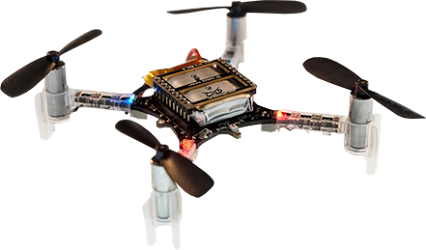
\includegraphics[width=.4\textwidth]{Images/crazyflie}
%\captionsetup[subfloat]{labelformat=empty}
%\subfloat[Picture from \cite{bitcraze}]{\hspace{\linewidth}}
%\caption{The CrazyFlie quadrotor from BitCraze}
%\label{fig:cf}
%\end{figure}

%%%%%%%%%%%%%%%%%%%%%%%%%%%%%%
%%%%%%%%%%% TWO FIGURES %%%%%%%%%%%
%%%%%%%%%%%%%%%%%%%%%%%%%%%%%%
%\begin{figure}[htbp]
%\centering
%\subfloat[Coarse Controller  ($K_p = 0.04,\  K_i = 0.008, \ K_d = 0.024$)]{\includegraphics[width=.45\textwidth]{Images/x_simple_PID}\label{fig:x_simple_PID_coarse}}
%\hspace{0.5cm}
%\subfloat[Fine Controller  ($K_p = 0.02,\  K_i = 0.004, \ K_d = 0.012$)]{\includegraphics[width=.45\textwidth]{Images/x_simple_PID_fine}\label{fig:x_simple_PID_fine}}
%\caption{X position for a simple PID controller}
%\label{fig:x_simple_PID}
%\end{figure}

%%%%%%%%%%%%%%%%%%%%%%%%%%%%%%
%%%%%%%%%%%%% TABLE %%%%%%%%%%%%%
%%%%%%%%%%%%%%%%%%%%%%%%%%%%%%
%\begin{table}[ht]
%\caption{X and Y controllers gains}
%\centering
%\begin{tabular}{|c|c|c|c|c|c|}
%\hline
%$\boldsymbol{K_{p,coarse}}$ & $\boldsymbol{K_{i,coarse}}$ & $\boldsymbol{K_{d,coarse}}$ &$\boldsymbol{K_{p,fine}}$ & $\boldsymbol{K_{i,fine}}$ & $\boldsymbol{K_{d,fine}}$ \\
%\hline
%0.04 & 0.008 & 0.024 & 0.02 & 0.004 & 0.024\\
%\hline
%\end{tabular}
%\label{tab:xy_param}
%\end{table}

%%%%%%%%%%%%%%%%%%%%%%%%%%%%%%
%%%%%%%%%%%%% CODE %%%%%%%%%%%%%
%%%%%%%%%%%%%%%%%%%%%%%%%%%%%%
%\lstset{
%commentstyle=\color{mygreen},
%stringstyle=\color{mymauve},
%keywordstyle=\color{blue},
%tabsize=2,
%frame=single,
%showstringspaces=false,
%basicstyle=\tiny
%}
%\lstinputlisting[language=Python]{Code/controlQuad.py}